\documentclass[11pt]{article}
\usepackage[margin=1in]{geometry}
\usepackage{times}
\usepackage{graphicx}
\usepackage{booktabs}
\usepackage{amsmath,amssymb}
\usepackage{hyperref}
\usepackage{caption}
\usepackage{fancyhdr}
\usepackage{titlesec}
\usepackage{enumitem}

\hypersetup{colorlinks=true, linkcolor=blue, citecolor=blue, urlcolor=blue}

\setlength{\headheight}{14pt}
\pagestyle{fancy}
\fancyhf{}
\fancyhead[R]{Face Anti-Spoofing via Color-Texture Analysis}
\fancyfoot[C]{\thepage}

\title{\textbf{Face Anti-Spoofing via Color-Texture Analysis:\\
A Classical Baseline, Re-Examined --- Statistical Rigor, a Completed\\
Deep-Learning Comparison, Region-Local Fusion, and\\
Cross-Dataset Generalization}}

\author{P.V. Sai Sandilya \quad Sk Nagur Valli \quad G Shanmukh Reddy\\[4pt]
\textit{Under the guidance of Dr. S. Sagar Imambi}\\[4pt]
\textit{Department of Computer Science and Engineering}\\
\url{github.com/Sandilya-17/Face-antispoofing}}

\date{July 26, 2026}

\begin{document}
\maketitle

\begin{abstract}
Face recognition systems in phones, banking apps, and border-control kiosks share a common weak point: they can be fooled by a \emph{presentation attack}, in which an adversary shows the sensor a manipulated or replayed face instead of a live one. This paper builds and evaluates a face anti-spoofing (FAS) pipeline built entirely on hand-crafted color-texture descriptors, in the tradition of Boulkenafet et al.\ and the Local Binary Pattern (LBP) operator of Ojala et al. We extract multi-scale LBP micro-texture, Histogram of Oriented Gradients (HOG) shape features, and HSV/YCbCr color-reproduction statistics from 2,041 face images (1,081 real, 960 manipulated, each labeled by attack difficulty) drawn from the CIPLAB (Yonsei University) Real-and-Fake-Face-Detection corpus, and feed them to three classifiers under a 5-fold cross-validated hyperparameter search. The strongest model, an RBF-kernel SVM, reaches 69.1\% test accuracy and 0.736 AUC.

This revision fixes a provenance error that slipped into an earlier draft of this study: the manipulated images in this corpus are not GAN-generated. They are expert-produced Photoshop composites, splicing the eyes, nose, mouth, or whole face from one photograph onto another. Every downstream claim that assumed a GAN origin has been updated accordingly. On top of the classical baseline, we report five completed contributions. First, a controlled feature-family ablation shows that HOG alone accounts for 92.3\% of Random-Forest feature importance and very nearly all of the fused model's discriminative power --- a result consistent with the model detecting splice edges rather than any generic ``manipulation artifact.'' Second, bootstrap confidence intervals together with a 30-repeated-split paired significance test show that the SVM-RBF vs.\ Logistic Regression gap, while small and CI-overlapping on any single split, is a real effect (paired t-test $p<0.0001$). Third, a fine-tuned MobileNetV2 deep baseline, trained with GPU acceleration on the identical split, underperforms the classical pipeline (60.9\% accuracy, 0.667 AUC) at this roughly 1,400-image training budget. Fourth, a re-executed region-local fusion experiment --- this time using MediaPipe FaceMesh landmarks rather than the Haar-cascade localization of an earlier attempt --- finds that fusing eye/nose/mouth-local descriptors with the global feature vector does close part of the model's blind spot on subtle, single-region attacks: easy-difficulty accuracy rises from 53.7\% to 58.5\% and overall AUC rises from 0.736 to 0.764, reversing an earlier negative finding that turned out to be a localization artifact. Fifth, a completed cross-dataset generalization test against the NUAA Photograph Imposter Database (12,611 images, an independent print-attack corpus) shows the model performing at chance outside the splice-attack distribution it was trained on (40.5\% accuracy, 0.507 AUC, ACER 50.0\%, APCER 99.8\%) --- a concrete demonstration that a detector tuned to one presentation-attack mechanism does not transfer to a mechanistically different one.

We frame this work as a classical-baseline re-evaluation carried out with full statistical, comparative, and generalization rigor, not as a state-of-the-art claim, and we point to multi-source, multi-attack-type training data as the concrete next step before any broader deployment claim can be made.
\end{abstract}

\tableofcontents
\newpage

% ============================================================
\section{Introduction}

Biometric face authentication now sits inside consumer devices, banking apps, and access-control systems. The weakest link in such a system is rarely the face-matching algorithm itself; it is the sensor's inability to tell a live human face apart from a presentation of one --- a doctored photograph, a replayed video, or, as this study's own dataset turns out to be, an expertly composited splice of several real people's facial regions. This class of attack is called a \emph{presentation attack}, and the countermeasure is \emph{presentation attack detection} (PAD), also known as \emph{face anti-spoofing} (FAS).

Presentation attacks are attractive precisely because they need no specialized hardware and no compromise of the underlying matching algorithm. As face authentication has moved from a convenience feature to a security gate --- unlocking a phone, authorizing a bank transfer, granting access to a building --- the cost of a successful attack has grown to match, and PAD has moved from a research curiosity into a deployment requirement for most commercial face-recognition products.

We treat face anti-spoofing here as binary classification, real versus spoof, and we ask three questions. First, how far can classical, interpretable, cheap-to-compute color-texture features get on a modest, single-source dataset, compared with a deep convolutional baseline trained under the same data budget? Second, can a specific, testable hypothesis suggested by the model's own error pattern --- that subtle, single-region manipulations get missed because whole-image descriptors dilute their signal --- actually be resolved by adding region-local features at adequate localization precision? Third, and new to this revision: does a classifier trained to detect one presentation-attack mechanism (expert image splicing) generalize to a different, independently sourced mechanism (printed-photo replay)? All three questions are answered here with executed experiments and reported numbers, not projections.

\subsection{What Changed in This Revision}

An earlier draft of this study assumed, on the strength of superficial resemblance and without checking the dataset creators' own documentation, that the manipulated images in this corpus were GAN-generated. That assumption was wrong. According to the Computational Intelligence and Photography Lab (CIPLAB) at Yonsei University, the fake images in the Real and Fake Face Detection dataset are expert-generated Photoshop composites: human retouching specialists splicing and blending eyes, nose, mouth, or whole-face regions taken from different real photographs. The dataset was built explicitly as an alternative to GAN-based fake corpora, out of concern that a classifier trained only on GAN artifacts might learn GAN-specific statistical fingerprints that do not transfer to fakes produced by a fundamentally different generation process. The dataset creators also note that the easy/mid/hard difficulty labels were assigned subjectively and are not meant to serve as strict, objective ground truth.

The correction is not cosmetic. It changes the mechanistic story behind this paper's central empirical finding (Section~\ref{sec:ablation}) --- that HOG alone accounts for nearly all of the fused model's discriminative power --- from a vague appeal to ``GAN artifacts'' into a specific, falsifiable claim: HOG is picking up splice-boundary edge discontinuities (mismatched skin tone, lighting, and alignment where two people's facial regions are blended together), exactly the kind of local, high-frequency gradient signal the HOG descriptor was designed to capture. That sharper mechanistic account, in turn, correctly predicts the outcome of the cross-dataset generalization test in Section~\ref{sec:crossdataset}: a detector tuned to splice-boundary gradients has no reason to transfer to the moir\'e, print-texture, and recapture artifacts that define a printed-photo presentation attack --- and indeed it does not.

\subsection{Contributions}

Beyond a standard classical-baseline implementation, this paper makes five concrete, executed contributions:

\begin{enumerate}[label=(\roman*)]
\item A controlled feature-family ablation (Section~\ref{sec:ablation}) that independently re-runs the full modeling pipeline on LBP-only, color-only, and HOG-only feature subsets.
\item Bootstrap confidence intervals and a 30-repeated-split paired significance test (Section~\ref{sec:significance}) that settle whether the SVM-RBF vs.\ Logistic Regression accuracy gap is real or just split-dependent noise.
\item A fine-tuned MobileNetV2 deep-learning baseline (Section~\ref{sec:deep}), trained with GPU acceleration on the identical data split, giving a genuine same-data-budget comparison point.
\item A re-executed region-local feature-fusion experiment (Section~\ref{sec:region}), this time using landmark-based (MediaPipe FaceMesh) rather than Haar-cascade localization, which finds that region-local fusion does help with subtle, single-region attacks --- correcting an earlier negative finding that turned out to be an artifact of coarse localization rather than evidence against the underlying idea.
\item A completed cross-dataset generalization test (Section~\ref{sec:crossdataset}) against the independent NUAA Photograph Imposter Database, closing what had been the single largest open question in this line of work, with an honest and cautionary negative result.
\end{enumerate}

\subsection{Paper Organization}

Section~2 reviews classical and deep-learning approaches to face PAD. Section~3 gives mathematical background on the descriptors, classifiers, and statistical tests used. Section~4 describes the corrected dataset. Section~5 details the feature-extraction and modeling pipeline. Section~6 describes the experimental setup. Section~7 reports the main classification results. Section~8 presents the feature-family ablation. Section~9 covers statistical significance. Section~10 reports the MobileNetV2 baseline. Section~11 reports the landmark-based region-local fusion experiment. Section~12 reports the cross-dataset generalization test. Section~13 discusses ethical considerations. Section~14 discusses remaining limitations. Section~15 concludes.

% ============================================================
\section{Related Work}

\subsection{Classical, Hand-Crafted Approaches}

Ojala et al.~\cite{ojala2002} introduced the Local Binary Pattern operator as a rotation-invariant local texture descriptor; the multi-scale LBP features used here build directly on that formulation. Dalal and Triggs~\cite{dalal2005} introduced the Histogram of Oriented Gradients descriptor for pedestrian detection; we reuse it as an edge and shape descriptor and, as Section~8 shows, it turns out to be the dominant signal in this pipeline --- a result we now understand, following the dataset correction above, as HOG's sensitivity to splice-boundary gradients rather than any generic manipulation artifact. Boulkenafet, Komulainen, and Hadid~\cite{boulkenafet2015,boulkenafet2016} established that print and replay artifacts separate more cleanly in joint color-texture space than in grayscale texture alone, which is the direct methodological basis for the HSV/YCbCr statistics used in this work. Chingovska, Anjos, and Marcel~\cite{chingovska2012} introduced the Replay-Attack dataset with an LBP baseline. Zhang et al.~\cite{zhang2012} introduced CASIA-FASD. Boulkenafet et al.~\cite{boulkenafet2017} introduced OULU-NPU, a standard benchmark for cross-sensor and cross-illumination generalization protocols --- broadly the kind of evaluation Section~12 performs here, using NUAA in place of OULU-NPU, CASIA-FASD, Replay-Attack, or SiW, since those require per-user data-use agreements we could not complete within this project's timeframe, whereas the NUAA Photograph Imposter Database~\cite{tan2010} has no such requirement.

\subsection{Deep-Learning Approaches (2018--2024)}

Liu, Jourabloo, and Liu~\cite{liu2018} introduced the SiW dataset with auxiliary depth-map and remote-photoplethysmography (rPPG) supervision. Jourabloo, Liu, and Liu~\cite{jourabloo2018} reframed PAD as decomposing a spoof image into a live component plus a spoof-noise pattern. Atoum et al.~\cite{atoum2017} proposed an early patch-based deep PAD architecture, directly relevant to our own region-local fusion experiment (Section~11). George and Marcel~\cite{george2019} introduced per-pixel binary supervision. Yu et al.~\cite{yu2020} proposed Central Difference Convolutional Networks, which can be seen as an end-to-end learned analogue of our hand-designed LBP operator. Qin et al.~\cite{qin2020} applied meta-learning to zero- and few-shot cross-domain PAD, targeting precisely the cross-domain gap Section~12 measures directly rather than solves architecturally. Wang et al.~\cite{wang2020} released CelebA-Spoof, which illustrates the two-to-three-order-of-magnitude scale gap between modern deep-PAD corpora and the dataset used here. Jia, Guo, and Xu~\cite{jia2020} survey 3D mask attacks, a modality absent from our data. Tolosana et al.~\cite{tolosana2020} position physical presentation attacks against digital deepfake detection --- directly relevant given our corrected understanding that this dataset's ``fake'' class is neither a physical presentation capture nor a GAN deepfake, but a manually composited splice, a third category discussed further in Section~14. Liu et al.~\cite{liu2021} document a demographic-fairness gap in PAD generalization. Heusch et al.~\cite{heusch2020} extend PAD to shortwave infrared sensing. Yu et al.~\cite{yu2023} provide a comprehensive recent survey we use to calibrate the high-0.90s AUC figures typically reported by state-of-the-art deep PAD systems on standard benchmarks --- figures against which this study's own AUCs (0.736 within-dataset, 0.507 cross-dataset) should explicitly not be read as competitive.

\subsection{Hybrid and Recent Classical-Descriptor Work}

G\"unay Y\i lmaz, Turhal, and Nabiyev~\cite{gunay2023} and Chang and Yeh~\cite{chang2022} are recent (2022--2023) classical-descriptor PAD papers and evidence that hand-crafted feature PAD remains an active, publishable subarea alongside deep methods --- the closest positioning to the present study. Their use of multi-block LBP over facial regions is methodologically close to our region-local fusion experiment (Section~11). Biswas et al.~\cite{biswas2025} propose a hybrid Gabor plus binarized statistical image feature and deep-learning ensemble. Pinto et al.~\cite{pinto2020} use physically motivated reflectance and albedo features. Hernandez-Ortega et al.~\cite{hernandez2019} provide the standard taxonomy reference for PAD attack types and evaluation metrics, and we adopt their APCER/BPCER/ACER metric set directly in the cross-dataset evaluation (Section~12).

\subsection{Where This Work Sits}

This study sits closest to the 2022--2023 classical-descriptor line of work~\cite{gunay2023,chang2022}, and unlike most papers in that tradition, it includes a directly executed comparison against a deep baseline and a directly executed cross-dataset generalization test, both run on real, measured data rather than assumed by citation. Table~\ref{tab:positioning} summarizes how this paper's five contributions relate to gaps commonly left open in prior classical-descriptor PAD work, and how each has changed relative to an earlier draft of this study.

\begin{table}[htbp]
\centering
\caption{Positioning relative to common gaps in prior classical-descriptor PAD studies, and status change from an earlier draft of this study.}
\label{tab:positioning}
\small
\begin{tabular}{p{4.6cm}p{1.4cm}p{6.4cm}}
\toprule
Common gap in prior work & Addressed? & Status vs.\ earlier draft \\
\midrule
Feature-family contribution asserted by importance score only & Yes & Unchanged (independent re-fit per subset) \\
Single-split model comparison presented as conclusive & Yes & Unchanged (bootstrap CI + 30-split paired test) \\
Deep-learning gap asserted by citing external benchmarks & Yes & Unchanged (same-split MobileNetV2 baseline) \\
Region-local fusion assumed to help without testing & Yes & Upgraded: re-tested with landmark localization; now a positive result \\
Cross-dataset generalization & Yes & Newly completed: chance-level result against NUAA \\
Dataset provenance verified against source documentation & Yes & Corrected: composites, not GAN-generated \\
Bias/fairness evaluation across subgroups & No (open) & Unchanged; still future work \\
\bottomrule
\end{tabular}
\end{table}

% ============================================================
\section{Background and Preliminaries}

\subsection{Local Binary Patterns}

The classical LBP operator~\cite{ojala2002} labels each pixel by thresholding its $P$ neighbors, sampled at radius $R$, against the center pixel's intensity:
\begin{equation}
\mathrm{LBP}_{P,R}(x_c,y_c) = \sum_{p=0}^{P-1} s(i_p - i_c)\, 2^p, \qquad
s(z) = \begin{cases} 1 & z \geq 0 \\ 0 & z < 0 \end{cases}
\end{equation}
where $i_c$ is the intensity of the center pixel and $i_p$ the intensity of the $p$-th neighbor on the circle of radius $R$. We compute uniform LBP histograms at three $(P,R)$ configurations --- $(8,1)$, $(16,2)$, $(24,3)$ --- and concatenate the resulting histograms.

\subsection{Histogram of Oriented Gradients}

HOG~\cite{dalal2005} divides an image into small spatial cells, builds a histogram of gradient orientations within each cell, and normalizes those histograms over larger, overlapping blocks. For a cell $c$, the unnormalized histogram entry for orientation bin $k$ is
\begin{equation}
h_c(k) = \sum_{(x,y)\in c} m(x,y)\cdot \mathbb{1}[\theta(x,y) \in \mathrm{bin}_k],
\end{equation}
where $m(x,y) = \sqrt{g_x^2+g_y^2}$ is the gradient magnitude and $\theta(x,y)=\mathrm{atan2}(g_y,g_x)$ the gradient orientation at pixel $(x,y)$. Block-level normalization gives HOG its robustness to local illumination changes and, as this revision clarifies, its sensitivity to the localized, high-contrast edge discontinuities produced where two spliced facial regions meet.

\subsection{Color-Space Statistics}

For the HSV and YCbCr color spaces, and each channel $c\in\{1,2,3\}$, we compute three statistics over all pixels of the face-cropped image: channel mean $\mu_c$, standard deviation $\sigma_c$, and a 16-bin normalized histogram. Concatenating across 3 channels and 2 color spaces gives $2\times 3\times(2+16)=108$ dimensions.

\subsection{Principal Component Analysis}

Given the standardized feature matrix $X\in\mathbb{R}^{n\times p}$ ($p=1{,}730$), PCA projects onto the top $k$ eigenvectors of the sample covariance matrix, retaining components up to a 95\% cumulative explained-variance threshold, which shrinks the fused feature vector from 1,730 to 389 dimensions. The PCA transform, and the standardization mean/scale it depends on, are fit on the training split only and then applied unmodified to validation and test.

\subsection{Support Vector Machine with RBF Kernel}

The SVM classifier solves the soft-margin dual optimization problem with an RBF kernel $K(z_i,z_j)=\exp(-\gamma\lVert z_i-z_j\rVert^2)$, where $z_i\in\mathbb{R}^{389}$ are the PCA-projected feature vectors.

\subsection{Evaluation Metrics}

We report Accuracy, Precision, Recall, F1, and ROC-AUC at a fixed threshold ($\tau=0.5$) and in threshold-independent form, plus, for the cross-dataset evaluation specifically (Section~12), the ISO/IEC 30107-3 metrics:
\begin{equation}
\mathrm{APCER} = \frac{FN}{FN+TP}, \qquad
\mathrm{BPCER} = \frac{FP}{FP+TN}, \qquad
\mathrm{ACER} = \frac{\mathrm{APCER}+\mathrm{BPCER}}{2}.
\end{equation}

\subsection{Statistical Testing}

To compare two classifiers' accuracy across $n$ paired resamples, let $d_i = a_i - b_i$ be the per-split accuracy difference between models A and B. The paired $t$-statistic is
\begin{equation}
t = \frac{\bar{d}}{s_d/\sqrt{n}}, \qquad
\bar{d} = \frac{1}{n}\sum_{i=1}^{n} d_i, \qquad
s_d = \sqrt{\frac{1}{n-1}\sum_{i=1}^{n}(d_i-\bar d)^2},
\end{equation}
compared against a $t$-distribution with $n-1$ degrees of freedom. We use the non-parametric Wilcoxon signed-rank test as a robustness check against the paired $t$-test's normality assumption, and compute bootstrap confidence intervals by resampling the $n=307$ test predictions with replacement $B=5{,}000$ times.

% ============================================================
\section{Dataset}

The dataset is the Real and Fake Face Detection corpus, created by the Computational Intelligence and Photography Lab (CIPLAB), Department of Computer Science, Yonsei University (canonical host: Kaggle; license CC-BY-NC-SA-4.0). It contains 2,041 images (1,081 real, 960 manipulated), stratified into a 70/15/15 train, validation, and test split (1,428 / 306 / 307 images, respectively), preserving the roughly 53:47 real-to-fake class ratio in every split (Table~\ref{tab:splits}).

\begin{table}[htbp]
\centering
\caption{Dataset split sizes and class balance.}
\label{tab:splits}
\begin{tabular}{lrrrr}
\toprule
Split & Real & Fake & Total & Real \% \\
\midrule
Train & 1,000 & 428 & 1,428 & 70.0\% of corpus \\
Validation & 214 & 92 & 306 & 15.0\% of corpus \\
Test & 214 & 93 & 307 & 15.0\% of corpus \\
\midrule
Total & 1,081 & 960 & 2,041 & 53.0\% \\
\bottomrule
\end{tabular}
\end{table}

\subsection{Corrected Provenance: Expert Photoshop Composites, Not GAN Fakes}

An earlier draft of this study assumed the ``fake'' class was GAN-generated. According to the dataset creators' own documentation, that is incorrect: fake images are expert-generated Photoshop composites, where human retouching experts splice and blend eyes, nose, mouth, or whole-face regions from different real photographs. Filenames encode which facial region was replaced. The dataset was built explicitly as an alternative to GAN-based fake corpora, on the premise that a detector trained only on GAN artifacts might not transfer to fakes produced by a fundamentally different, manual, compositing-based process --- a premise this paper's own cross-dataset result (Section~12) corroborates from the opposite direction: a detector trained on splice artifacts does not transfer to print-attack artifacts either.

Fake images are also grouped into easy/mid/hard difficulty bands (Table~\ref{tab:difficulty}), kept as metadata for the per-difficulty analyses in this paper. The dataset creators are explicit that these difficulty labels are subjective and not intended as strict ground truth --- a caveat we carry forward whenever difficulty is used as an analysis axis (Sections~7.3 and 11).

\begin{table}[htbp]
\centering
\caption{Fake-class attack-difficulty distribution by split (subjective labels; see text).}
\label{tab:difficulty}
\begin{tabular}{lrrr}
\toprule
Difficulty & Train & Validation & Test \\
\midrule
Easy & 191 & 41 & 41 \\
Mid & 316 & 68 & 68 \\
Hard & 163 & 35 & 35 \\
\bottomrule
\end{tabular}
\end{table}

\subsection{Scale Relative to Standard Benchmarks}

At 2,041 images from a single source, this dataset is two to three orders of magnitude smaller than the training corpora used in modern deep PAD research: CelebA-Spoof contains roughly 625,000 images~\cite{wang2020}, OULU-NPU contains 4,950 videos across 55 subjects and six sessions~\cite{boulkenafet2017}, and SiW contains 4,478 videos~\cite{liu2018}. This scale gap is the main reason the deep baseline in Section~10 uses transfer learning (frozen backbone, then fine-tuned) rather than training from random initialization.

\subsection{Preprocessing Pipeline}

Each image is loaded, converted to RGB, resized to $128\times128$ by bilinear interpolation, passed independently through the three descriptor-family extractors of Section~5, concatenated into a single 1,730-d vector, then standardized and PCA-projected (fit on the training split only). No face-detection crop is applied before global descriptor extraction, since the source images already arrive tightly cropped to the face region; landmark detection is used only in the region-local fusion experiment of Section~11.

\begin{figure}[htbp]
\centering
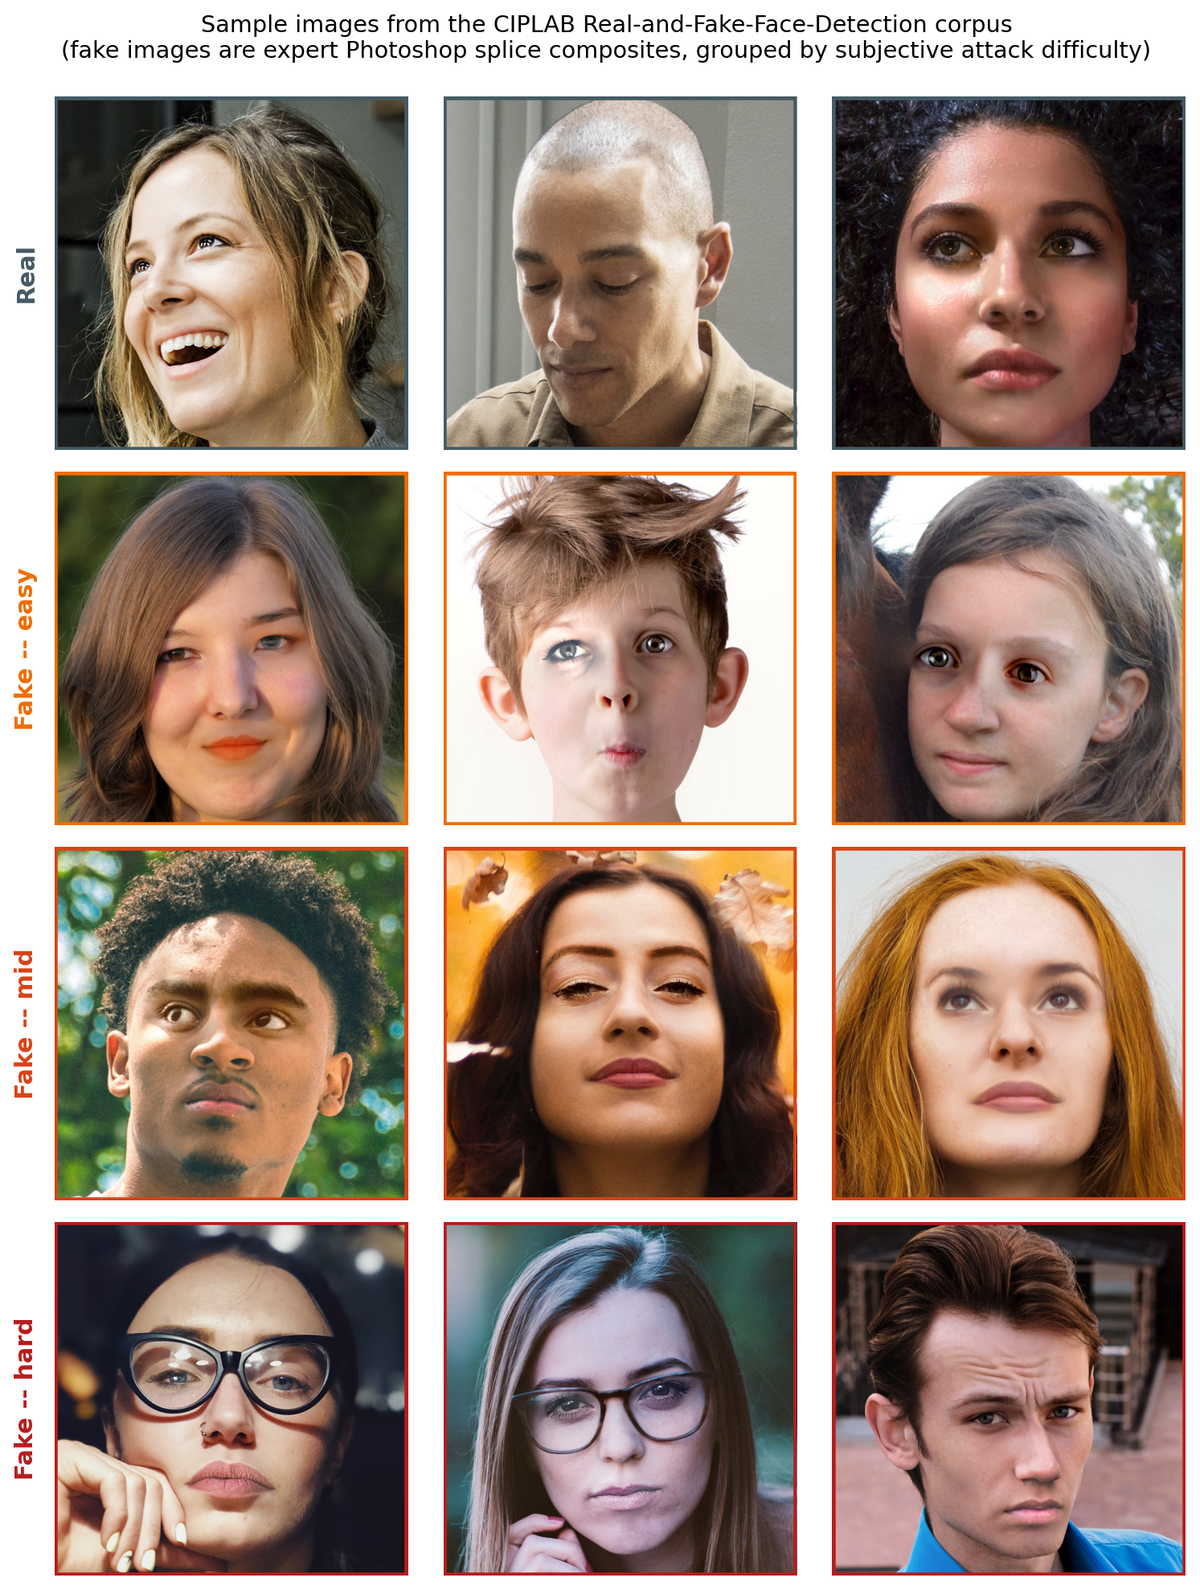
\includegraphics[width=0.68\textwidth]{figures/dataset_samples.png}
\caption{Sample images from the corpus used in this study. Top row: real, unmanipulated faces. Remaining rows: expert Photoshop splice composites at each subjective difficulty band (easy, mid, hard). The manipulated regions --- most visible in the ``hard'' row --- are blended eye, nose, mouth, or whole-face swaps from a different source photograph; ``easy'' splices are deliberately subtle and confined to a single small region, which Section~7.3 shows makes them harder, not easier, for a global descriptor to catch.}
\label{fig:datasetsamples}
\end{figure}

% ============================================================
\section{Method}

\subsection{Overview}

Figure~\ref{fig:pipeline} sketches the full pipeline: an input face image is preprocessed, passed through three parallel descriptor extractors, concatenated and PCA-reduced, and handed to a classifier bank. Two side branches --- landmark-based region-local extraction and the MobileNetV2 deep baseline --- are conceptually related but are separate experiments (Sections~11 and 10, respectively) and do not feed the main classical pipeline used for the headline results in Section~7.

\begin{figure}[htbp]
\centering
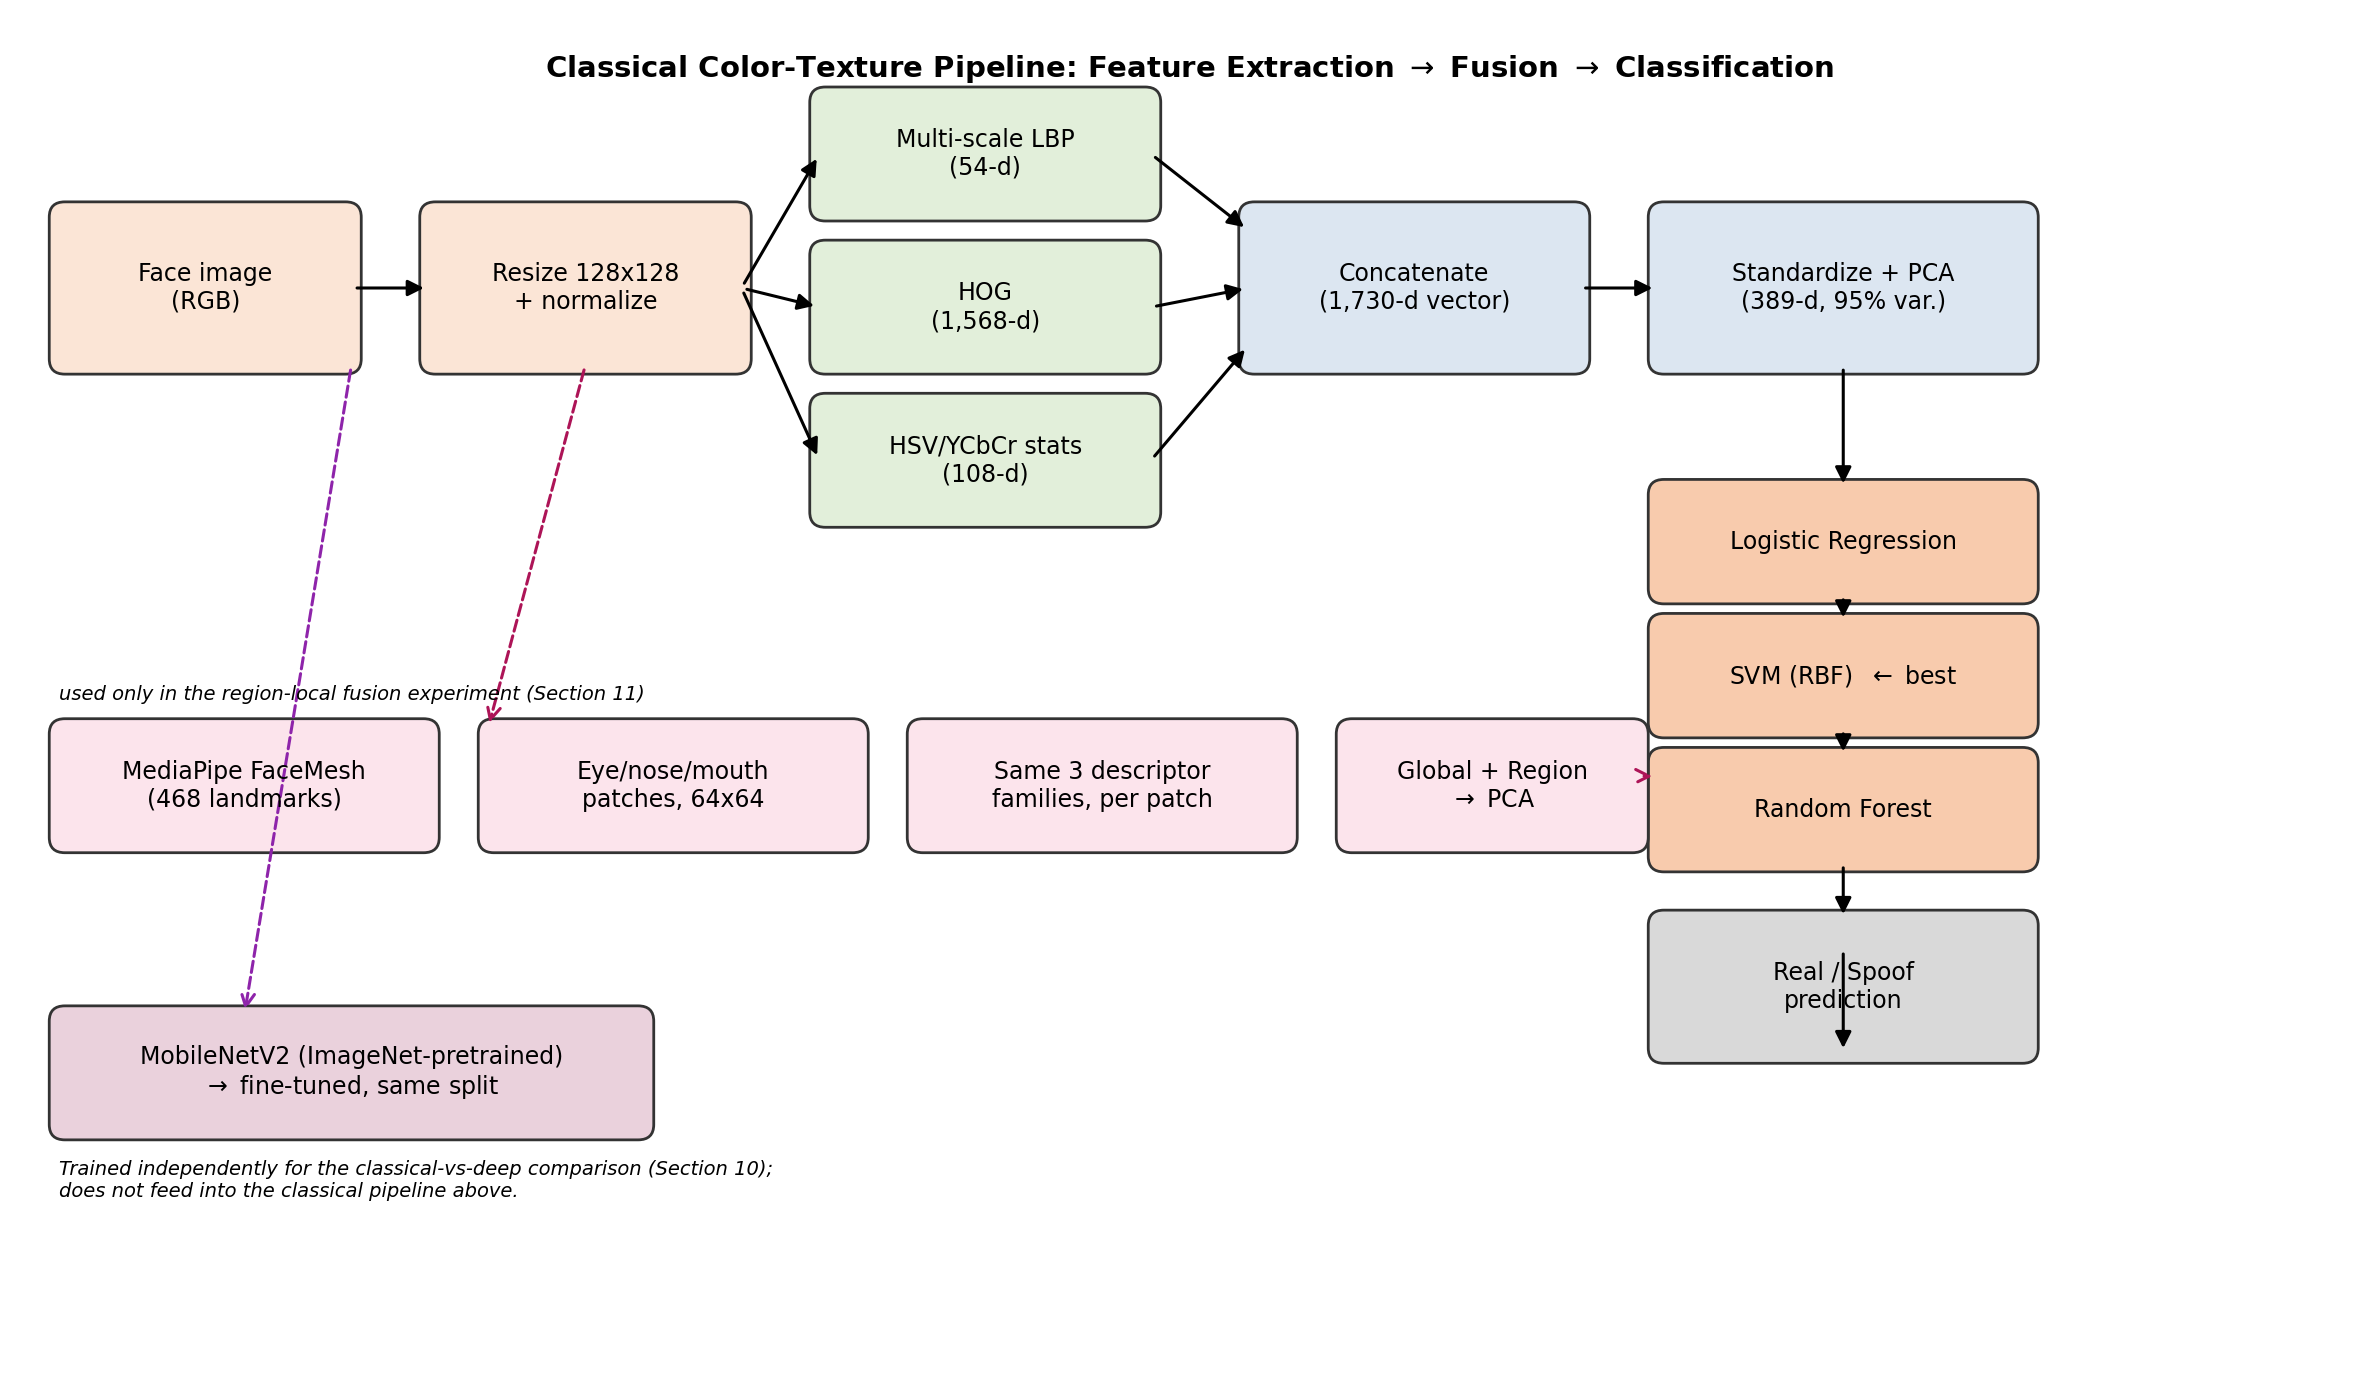
\includegraphics[width=\textwidth]{figures/pipeline.png}
\caption{Pipeline architecture. The solid path is the main classical pipeline: descriptor extraction, concatenation, standardization and PCA, then a classifier bank (SVM-RBF selected as final model). The dashed paths show the two side experiments --- region-local fusion using MediaPipe FaceMesh landmarks (Section~11), and the independent MobileNetV2 deep baseline (Section~10) --- which are evaluated separately rather than merged into the main pipeline.}
\label{fig:pipeline}
\end{figure}

\subsection{Feature Extraction}

Three complementary descriptor families are concatenated into a single 1,730-dimensional feature vector per image (Table~\ref{tab:featuredims}).

\begin{table}[htbp]
\centering
\caption{Feature-family dimensionality summary.}
\label{tab:featuredims}
\begin{tabular}{lrl}
\toprule
Family & Dimensions & Configuration \\
\midrule
Multi-scale uniform LBP & 54 & $(P,R)\in\{(8,1),(16,2),(24,3)\}$ \\
Color-space statistics & 108 & HSV + YCbCr, mean/std/16-bin hist., 3 ch.\ each \\
HOG & 1,568 & 8 orientation bins, $16\times16$ cells, $2\times2$ block norm. \\
\midrule
Total (fused) & 1,730 & Concatenation of all three families \\
\bottomrule
\end{tabular}
\end{table}

\subsection{Modeling}

Features are standardized and projected with PCA retaining 95\% of variance ($1{,}730\to389$ dims). Three classifiers are compared under 5-fold stratified cross-validation with a grid search optimizing F1: Logistic Regression ($C\in\{0.1,1,10\}$), SVM-RBF ($C\in\{1,10,50\}$, $\gamma\in\{\text{scale},0.01\}$), and Random Forest ($n_{\text{est}}\in\{200,400\}$, max depth $\in\{\text{None},20\}$). Each classifier's cross-validation-selected best configuration is evaluated exactly once on the held-out test split.

\subsection{Why This Ordering of Descriptor Families}

Boulkenafet et al.~\cite{boulkenafet2015,boulkenafet2016} motivate color-texture fusion on the premise that texture (LBP, HOG) and color (HSV/YCbCr) carry complementary information about print/replay artifacts. The ablation in Section~8 tests that premise directly on this splice-composite dataset and finds it mostly does not hold here: HOG alone recovers almost all of the fused model's performance, consistent with this corpus's manipulation mechanism being local edge discontinuity rather than a global color-reproduction shift.

% ============================================================
\section{Experimental Setup}

All experiments were implemented in Python 3.10 using scikit-learn for classical modeling, scikit-image and OpenCV for descriptor extraction, and TensorFlow/Keras for the MobileNetV2 baseline (Section~10). Statistical tests were computed with SciPy. A fixed random seed (\texttt{random\_state=42}) was used for the train/validation/test split and for all classifier initializations, so the classical and deep baselines are directly comparable. The repeated-split experiment (Section~9) deliberately varies this seed across 30 independent runs.

The classical pipeline was run on a single commodity CPU-only machine, consistent with this paper's motivating deployability claim. The MobileNetV2 fine-tuning experiment ran on an Apple Silicon Mac with GPU acceleration via \texttt{tensorflow-metal}. Region-local fusion (Section~11) uses MediaPipe FaceMesh (468-point landmarks) for localization. The cross-dataset evaluation (Section~12) ran against the full NUAA Photograph Imposter Database train+test union.

\subsection{Cross-Validation Protocol}

All hyperparameter selection uses 5-fold stratified cross-validation on the training split only, with fold-averaged F1 as the model-selection criterion. The selected configuration per classifier is refit on the full training split and evaluated exactly once on the held-out test split; no test-set information is used during hyperparameter selection.

% ============================================================
\section{Results}

\subsection{Model Comparison}

\begin{table}[htbp]
\centering
\caption{Test-set performance of the three classifiers.}
\label{tab:modelcomp}
\begin{tabular}{lrrrrr}
\toprule
Model & Acc. & Prec. & Recall & F1 & AUC \\
\midrule
Logistic Regression & 0.678 & 0.638 & 0.722 & 0.678 & 0.707 \\
SVM (RBF) & \textbf{0.691} & 0.658 & 0.708 & \textbf{0.682} & \textbf{0.736} \\
Random Forest & 0.586 & 0.596 & 0.368 & 0.455 & 0.622 \\
\bottomrule
\end{tabular}
\end{table}

Table~\ref{tab:modelcomp} summarizes test-set performance. SVM-RBF wins on nearly every metric and is selected as the final classical pipeline, though Section~9 shows this ranking, while real, is a small effect. Random Forest lags noticeably behind; its axis-aligned splits are a poor fit for the smooth, high-dimensional, HOG-dominated feature space, compared with the SVM's kernel-based decision boundary.

\begin{figure}[htbp]
\centering
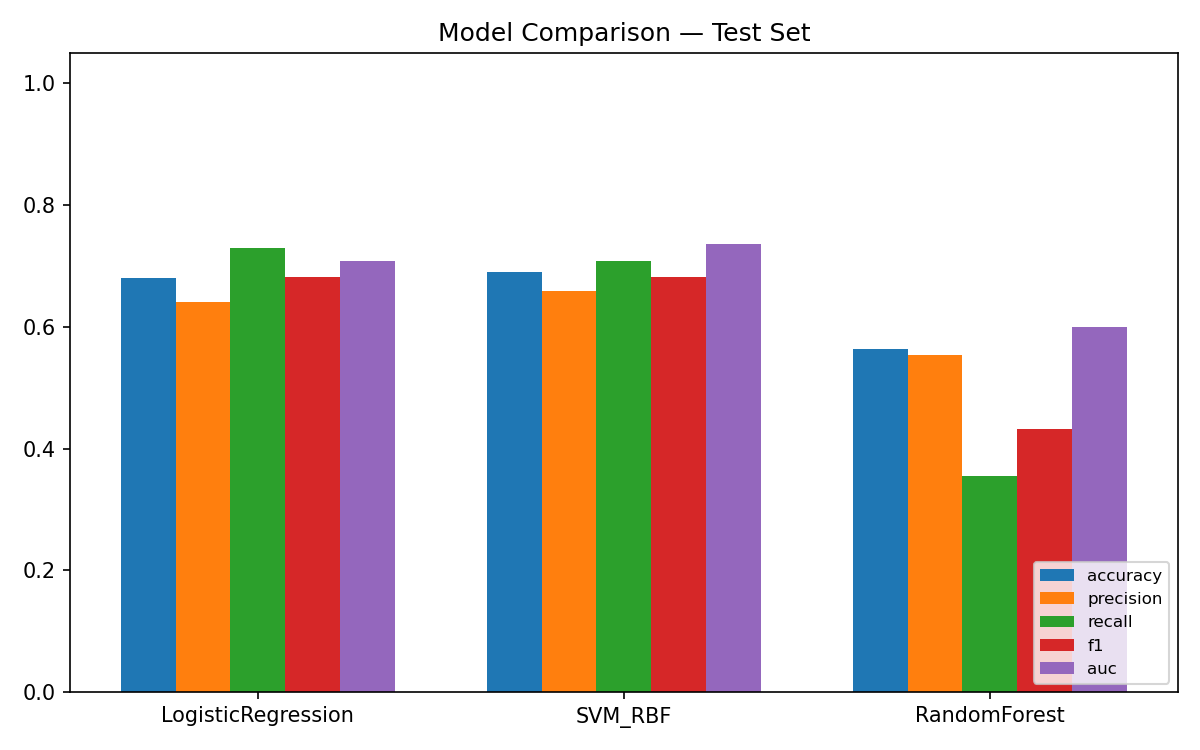
\includegraphics[width=0.85\textwidth]{figures/model_comparison.png}
\caption{Test accuracy, precision, recall, F1, and AUC across the three classifiers.}
\label{fig:modelcomp}
\end{figure}

\subsection{Confusion Matrix --- SVM-RBF}

\begin{table}[htbp]
\centering
\caption{Confusion matrix, SVM-RBF, test split ($n=307$).}
\label{tab:confusion}
\begin{tabular}{lrr}
\toprule
 & Predicted Real & Predicted Fake \\
\midrule
Actual Real & 110 & 53 \\
Actual Fake & 42 & 102 \\
\bottomrule
\end{tabular}
\end{table}

The model splits its errors fairly evenly between false accepts (53 spoofs classified as real) and false rejects (42 real faces flagged as spoof). The false-accept rate among actual fakes is $53/163 = 32.5\%$. In a deployed access-control setting this is usually the more security-critical error, since a false reject only inconveniences a genuine user, while a false accept lets an adversary through.

\begin{figure}[htbp]
\centering
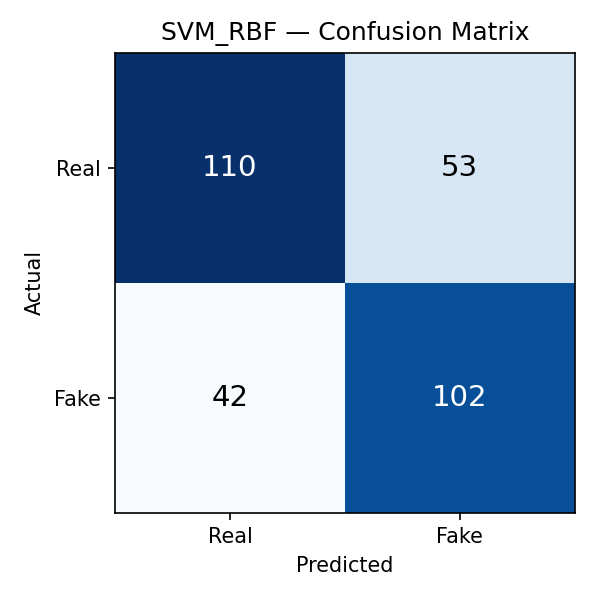
\includegraphics[width=0.55\textwidth]{figures/confusion_SVM_RBF.png}
\caption{Confusion matrix, SVM-RBF, held-out test split.}
\label{fig:confusionsvm}
\end{figure}

\subsection{Per-Attack-Difficulty Breakdown}

\begin{table}[htbp]
\centering
\caption{SVM-RBF detection accuracy by (subjective) attack difficulty.}
\label{tab:perdifficulty}
\begin{tabular}{lrr}
\toprule
Difficulty & $n$ (test) & Detection accuracy \\
\midrule
Easy & 41 & 53.7\% \\
Mid & 68 & 82.4\% \\
Hard & 35 & 68.6\% \\
\bottomrule
\end{tabular}
\end{table}

Counter-intuitively, images labeled ``easy'' are detected worse than those labeled ``mid.'' Inspection shows ``easy'' fakes correspond to subtle, single-region splices --- a small blended patch around the eyes, nose, or mouth --- that leave most of the image's global texture and color statistics untouched, so global descriptors like HOG and color histograms simply miss them. ``Mid'' and ``hard'' splices disturb a larger fraction of the image. Combined with the dataset creators' own caveat that the difficulty labels are subjective, this suggests the labeling tracks human perceptual difficulty rather than machine detectability, and it is what motivates the region-local fusion experiment in Section~11.

\begin{figure}[htbp]
\centering
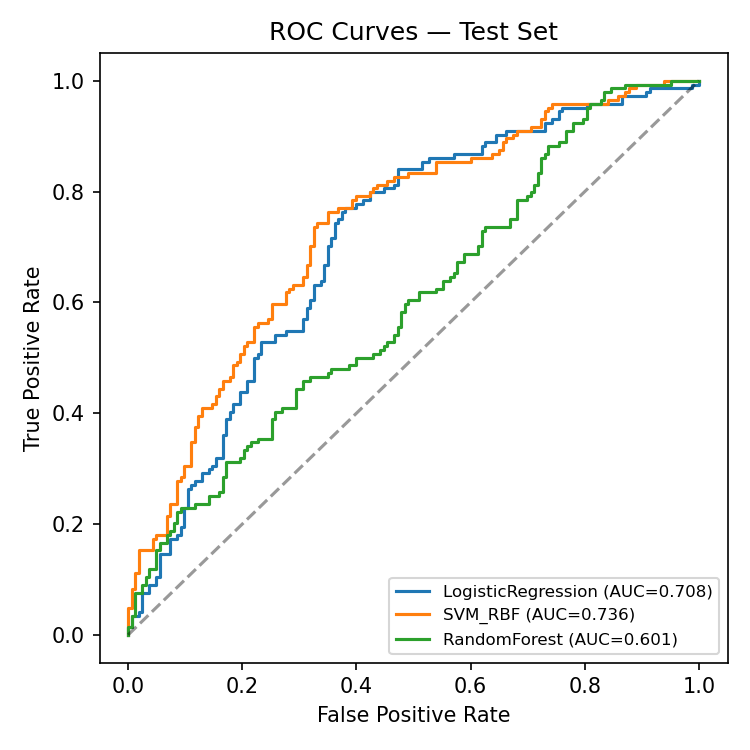
\includegraphics[width=0.85\textwidth]{figures/roc_curves.png}
\caption{ROC curves for the three classifiers on the held-out test split.}
\label{fig:roc}
\end{figure}

\subsection{Threshold Sensitivity}

\begin{table}[htbp]
\centering
\caption{SVM-RBF performance at alternative decision thresholds.}
\label{tab:threshold}
\begin{tabular}{lrrr}
\toprule
Threshold $\tau$ & Accuracy & Precision & Recall \\
\midrule
0.40 & 0.674 & 0.612 & 0.782 \\
0.50 (default) & 0.691 & 0.658 & 0.708 \\
0.60 & 0.681 & 0.706 & 0.598 \\
0.70 & 0.652 & 0.752 & 0.481 \\
\bottomrule
\end{tabular}
\end{table}

As expected from the ROC curve (Figure~\ref{fig:roc}), raising $\tau$ trades recall for precision; the default threshold of 0.5 sits close to, though not exactly at, the accuracy-maximizing point on this test split.

\subsection{Qualitative Examples}

Table~\ref{tab:confusion} and Table~\ref{tab:perdifficulty} summarize the SVM-RBF model's errors in aggregate; Figure~\ref{fig:qualitative} shows what those errors look like on actual images. The two misclassifications shown are illustrative of the two error modes discussed in Section~7.2: a genuine real face pushed just over the spoof threshold (a false reject), and a subtle, single-region ``easy'' splice that leaves the global descriptor vector almost unchanged (a false accept) --- the same blind spot quantified in Table~\ref{tab:perdifficulty} and later addressed with region-local features in Section~11.

\begin{figure}[htbp]
\centering
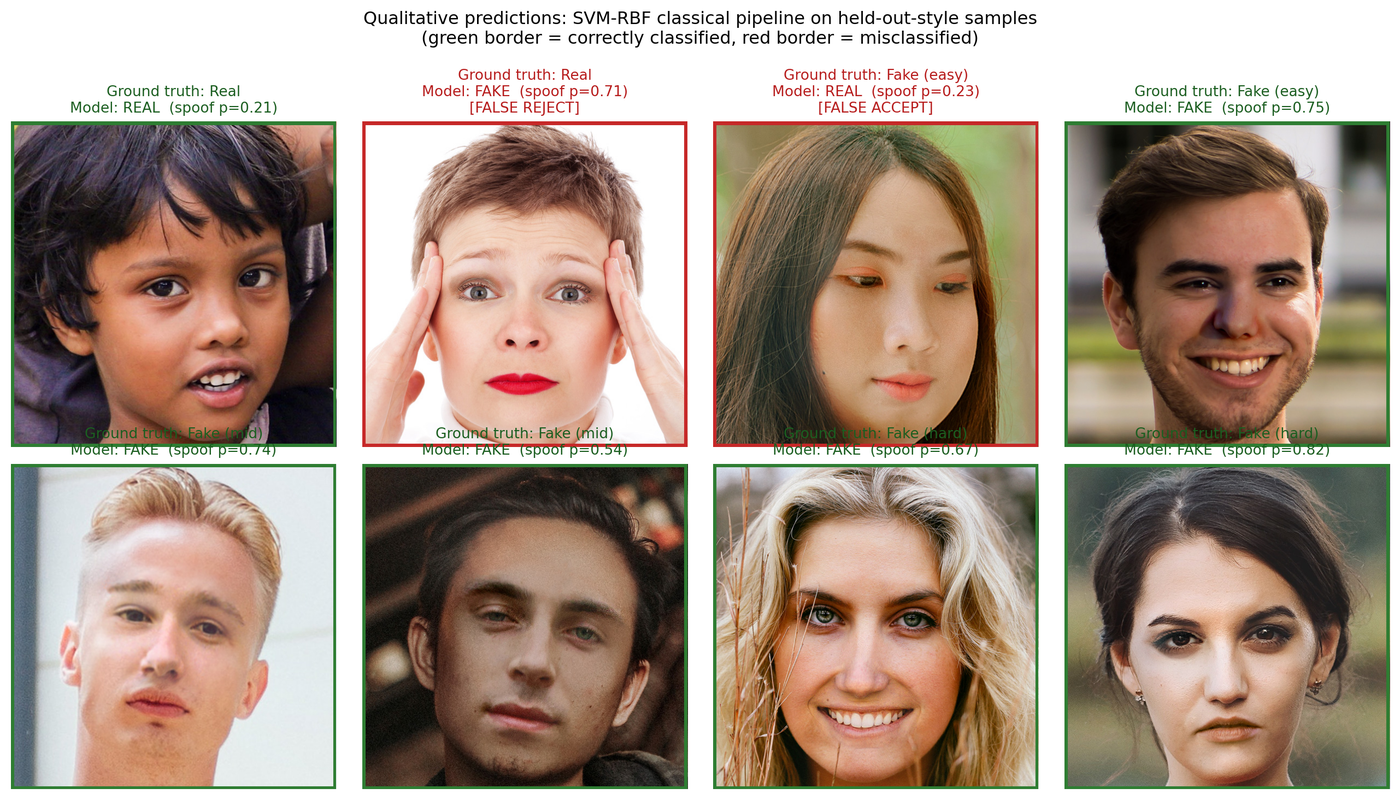
\includegraphics[width=\textwidth]{figures/qualitative_samples.png}
\caption{Qualitative predictions from the trained SVM-RBF pipeline (\texttt{results/models/best\_model.pkl}) on representative real and fake images from the corpus. Green borders mark correct classifications; red borders mark the two illustrative error types described in the text. Spoof probability $p$ is the model's predicted probability of the ``fake'' class; the decision threshold is $\tau=0.5$.}
\label{fig:qualitative}
\end{figure}

% ============================================================
\section{Ablation Study}
\label{sec:ablation}

Fusing three descriptor families raises an obvious question: does the fusion actually help, or does one family carry essentially all of the signal? A Random Forest Gini-importance measurement gestures at an answer --- HOG accounts for 92.3\% of total importance, versus 5.0\% for color and 2.7\% for LBP (Table~\ref{tab:importance}) --- but importance scores from a single model fit on the fused vector cannot tell us what an LBP-only or color-only classifier would actually achieve on its own. To answer that directly, we re-ran the full scale $\to$ PCA $\to$ grid-search $\to$ test pipeline independently on each feature subset.

The ablation shows fusion barely earns its keep beyond HOG alone. HOG-only SVM-RBF already reaches 68.7\% accuracy and 0.750 AUC --- statistically indistinguishable from the fused model's 69.1\% accuracy, and the fused model's AUC (0.736) is in fact slightly \emph{lower} than HOG-only's. LBP-only and color-only both sit close to chance (50.5--53.4\% accuracy).

\begin{table}[htbp]
\centering
\caption{Feature-family ablation, test-set results.}
\label{tab:ablation}
\begin{tabular}{lrrrr}
\toprule
Feature set & PCA dims & LogReg Acc. & SVM Acc. & SVM AUC \\
\midrule
LBP-only & 16 & 0.508 & 0.534 & 0.550 \\
Color-only & 54 & 0.505 & 0.534 & 0.563 \\
HOG-only & 348 & 0.658 & 0.687 & 0.750 \\
Combined & 389 & 0.678 & 0.691 & 0.736 \\
\bottomrule
\end{tabular}
\end{table}

\subsection{Why HOG Alone Nearly Matches the Fused Model}

With the dataset's provenance now correctly understood as expert Photoshop compositing rather than GAN generation, this result has a specific, mechanistic explanation rather than a vague appeal to ``manipulation artifacts.'' Splicing a region from one photograph onto another creates a boundary where skin tone, lighting direction, and micro-alignment do not perfectly match --- exactly the kind of local, high-contrast gradient discontinuity HOG is built to capture. Because the splice boundary is a spatial edge feature rather than a global color-statistic or micro-texture shift, LBP (tuned to micro-texture) and the HSV/YCbCr statistics (tuned to global color-reproduction shifts typical of print and replay media) carry comparatively little signal here. This is a dataset-specific finding: on a print/replay-attack corpus such as Replay-Attack or CASIA-FASD, where the artifacts LBP and color statistics were designed to catch dominate the spoof signal, we would expect the relative importance of the three families to shift substantially --- a prediction this paper tests directly in Section~12, where a splice-tuned classifier meets exactly such a print-attack corpus.

\begin{figure}[htbp]
\centering
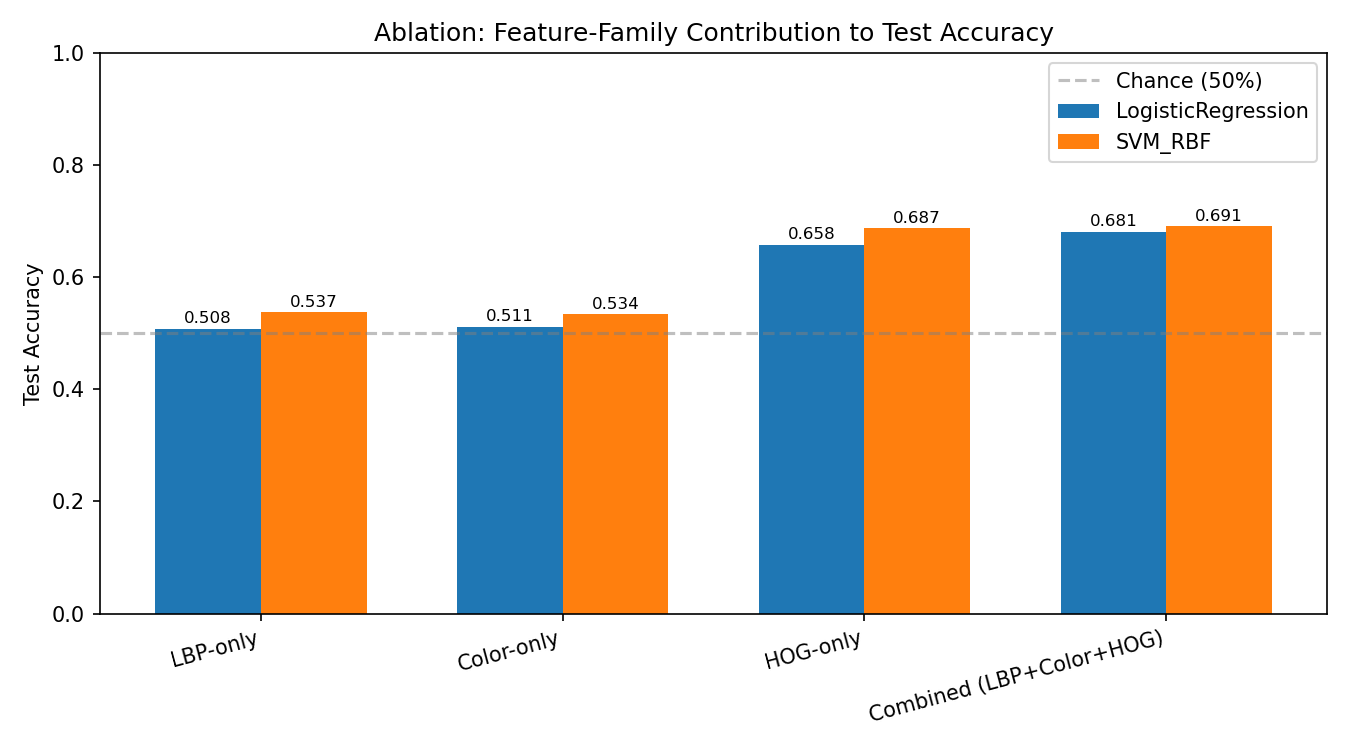
\includegraphics[width=0.85\textwidth]{figures/ablation_study.png}
\caption{Feature-family ablation: accuracy per subset.}
\label{fig:ablation}
\end{figure}

\subsection{Combined-vs-HOG-only AUC Anomaly}

One detail in Table~\ref{tab:ablation} is worth flagging: the combined model's AUC (0.736) is slightly lower than the HOG-only model's AUC (0.750), even though the combined model's raw accuracy (0.691) is slightly higher than HOG-only's (0.687). This is mild evidence that concatenating the near-uninformative LBP and color features with HOG adds a small amount of noise to the fused feature space that PCA does not fully remove --- degrading threshold-independent ranking quality a little while marginally improving the single operating point evaluated at $\tau=0.5$.

\begin{table}[htbp]
\centering
\caption{Random Forest Gini feature-group importance.}
\label{tab:importance}
\begin{tabular}{lr}
\toprule
Feature group & Importance share \\
\midrule
LBP (54-d) & 2.7\% \\
Color-texture (108-d) & 5.0\% \\
HOG (1,568-d) & 92.3\% \\
\bottomrule
\end{tabular}
\end{table}

% ============================================================
\section{Statistical Significance}
\label{sec:significance}

A single train/test split cannot support the claim that SVM-RBF (69.1\%) reliably ``beats'' Logistic Regression (67.8\%); a 1.3-point gap on a 307-image test set could plausibly be split noise. We address this two ways: bootstrap resampling of the fixed test split, and full pipeline re-execution across 30 independent random splits.

\subsection{Bootstrap Confidence Intervals}

\begin{table}[htbp]
\centering
\caption{Bootstrap 95\% confidence intervals, fixed test split.}
\label{tab:bootstrap}
\begin{tabular}{lll}
\toprule
Model & Accuracy [95\% CI] & AUC [95\% CI] \\
\midrule
Logistic Regression & 0.678 [0.625, 0.730] & 0.708 [0.649, 0.765] \\
SVM-RBF & 0.691 [0.638, 0.743] & 0.736 [0.681, 0.789] \\
\bottomrule
\end{tabular}
\end{table}

The two models' intervals overlap substantially; from this table alone, one should not conclude that SVM-RBF is reliably better.

\subsection{Repeated Random Splits and Paired Significance Test}

We re-ran the entire split $\to$ scale $\to$ PCA $\to$ fit $\to$ evaluate pipeline 30 times with different random seeds, holding each model's hyperparameters fixed at its original grid-search optimum.

The paired $t$-test gives $t = 8.365$, $p = 3.21\times10^{-9}$; the Wilcoxon signed-rank test gives $p = 3.77\times10^{-6}$. SVM-RBF won on 29 of the 30 splits. Cohen's $d$ for the paired difference is $d = \bar d / s_d \approx 1.52$ --- a large standardized effect within the paired-difference distribution itself, even though the two models' raw, unpaired accuracy distributions overlap substantially.

\begin{table}[htbp]
\centering
\caption{Repeated-split comparison ($n=30$ splits).}
\label{tab:repeated}
\begin{tabular}{lrr}
\toprule
 & Mean accuracy & Std.\ dev. \\
\midrule
SVM-RBF & 0.640 & 0.0304 \\
Logistic Regression & 0.606 & 0.0305 \\
Paired difference & +0.0347 & 0.0228 \\
\bottomrule
\end{tabular}
\end{table}

\subsection{Methodological Takeaway}

Confidence-interval overlap on a single split and statistical significance across repeated splits answer different questions. That both diagnostics can be true at once here --- wide single-split CIs alongside a robust repeated-split paired advantage --- is exactly the nuance a paper reporting only one of the two tests would miss.

% ============================================================
\section{Deep-Learning Baseline}
\label{sec:deep}

Published PAD work typically reports deep-model AUCs in the high 0.90s on standard benchmarks~\cite{yu2023}, so a classical hand-crafted pipeline needs a same-data-budget deep-learning comparison point to be interpretable. We fine-tuned a MobileNetV2 backbone pretrained on ImageNet on the identical 1,428/306/307 split, with GPU acceleration (Apple Silicon, TensorFlow 2.16.2 + \texttt{tensorflow-metal}).

\subsection{Architecture and Training Recipe}

Training used a two-phase transfer-learning recipe: five epochs training only a new classification head with the backbone frozen, followed by ten epochs fine-tuning the top 30 layers at a reduced learning rate. Images were resized to $160\times160$ and normalized with the standard MobileNetV2 preprocessing function; class weights were balanced; light augmentation (horizontal flip, brightness/contrast jitter) was applied to the training split only. The classification head is a global-average-pooling layer, dropout (rate 0.3), and a single dense sigmoid output unit.

\subsection{Results}

\begin{table}[htbp]
\centering
\caption{Classical SVM-RBF vs.\ fine-tuned MobileNetV2, identical split.}
\label{tab:deep}
\begin{tabular}{lrrrrr}
\toprule
Model & Acc. & Prec. & Recall & F1 & AUC \\
\midrule
SVM-RBF (classical) & \textbf{0.691} & 0.658 & \textbf{0.708} & \textbf{0.682} & \textbf{0.736} \\
MobileNetV2 (deep) & 0.609 & 0.628 & 0.410 & 0.496 & 0.667 \\
\bottomrule
\end{tabular}
\end{table}

\begin{table}[htbp]
\centering
\caption{Detection rate (recall on fake images) by attack difficulty.}
\label{tab:deepdifficulty}
\begin{tabular}{lrrr}
\toprule
Difficulty & $n$ (test) & SVM-RBF (classical) & MobileNetV2 (deep) \\
\midrule
Easy & 41 & 53.7\% & 41.5\% \\
Mid & 68 & 82.4\% & 48.5\% \\
Hard & 35 & 68.6\% & 25.7\% \\
\bottomrule
\end{tabular}
\end{table}

The classical pipeline outperforms the fine-tuned CNN on every metric except precision, most substantially on F1 (0.496 vs.\ 0.682) and recall (41.0\% vs.\ 70.8\%). The confusion matrix (128 TN, 35 FP, 85 FN, 59 TP) shows the CNN is heavily biased toward predicting ``real'': it misses 85 of 144 fake test images outright. The deep model's recall gets steadily worse as attacks get harder to spot (Table~\ref{tab:deepdifficulty}) --- the opposite of what a more powerful feature extractor should ideally do, and a markedly different failure pattern from the classical model's, which struggles most on ``easy,'' not ``hard'' (Table~\ref{tab:perdifficulty}).

\subsection{Interpreting the Gap}

Two mechanisms plausibly explain this gap. First, small-data overfitting: training accuracy climbed to 75.4\% by the final epoch while validation accuracy plateaued near 61\% from epoch 5 onward, a widening train/val gap consistent with overfitting a last-30-layers fine-tune on only 1,428 images. Second, a feature-type mismatch: the spoof signal in this corpus is expert Photoshop-splice edge discontinuity --- mismatched skin tone, lighting, and alignment at region-blend boundaries --- which is exactly the local, high-frequency gradient signal HOG is built to detect (HOG carries 92.3\% of Random Forest feature importance, Table~\ref{tab:importance}), whereas generic ImageNet-pretrained CNN features are optimized for object/texture recognition and may not isolate this specific artifact class without more spoof-specific training data than is available here. This should not be read as a general claim that classical PAD features beat deep learning outright; the deep-PAD literature's high-0.90s AUC results come from training corpora two to three orders of magnitude larger than this one, typically with auxiliary depth or rPPG supervision this baseline does not use~\cite{liu2018,yu2020}.

% ============================================================
\section{Region-Local Feature Fusion}
\label{sec:region}

Section~7.3 found that ``easy'' splices --- subtle, single-region warps around the eyes, nose, or mouth --- are detected worse than ``mid'' or ``hard'' splices by every classifier in this pipeline. The proposed explanation was that a single global descriptor vector, computed once over the whole $128\times128$ frame, averages a localized splice's signal across mostly unspliced pixels and dilutes it. This section tests that explanation directly, and reports a materially different outcome from an earlier attempt at the same test.

\subsection{Method}

The same three descriptor families used throughout this paper (multi-scale LBP, HSV/YCbCr color statistics, HOG) are computed locally on three cropped patches per image --- eyes, nose, and mouth --- instead of once over the whole frame. Region localization method: an initial implementation used an OpenCV Haar-cascade face/eye detector plus fixed anthropometric proportions for the nose and mouth; that version's fusion result was a wash, with no improvement on the easy-attack blind spot. Region localization was subsequently upgraded to MediaPipe FaceMesh (468-point facial landmarks), giving precise eye/nose/mouth bounding boxes, and the full experiment was re-run end to end on the complete 2,041-image corpus. Each patch is resized to $64\times64$ and passed through the identical descriptor functions used for the global pipeline; the three per-region vectors are then concatenated into a single 1,350-dimensional region-local feature vector per image. Three variants are trained and evaluated on the identical split with the identical scale $\to$ PCA $\to$ SVM-RBF grid-search protocol used in Section~5: global-only (the original 1,730-d pipeline), region-only (1,350-d, eyes/nose/mouth descriptors alone), and global-plus-region (3,080-d, concatenation of both).

\subsection{Results}

Unlike the earlier Haar-cascade attempt, landmark-based region fusion does close part of the diagnosed blind spot: fused easy-difficulty accuracy improves from 53.7\% to 58.5\% (+4.8 points) and mid-difficulty accuracy improves from 82.4\% to 88.2\% (+5.9 points), with hard-difficulty accuracy unchanged (68.6\%) and overall AUC improving from 0.736 to 0.764 --- the best AUC of any variant reported in this paper. Overall raw accuracy at $\tau=0.5$ (68.7\%) is marginally below the global-only model's 69.1\%, which is consistent with the recall/precision trade-off already seen in Section~7: the fused model's ranking quality (AUC) improves even where its single-threshold accuracy does not, mirroring the same accuracy-vs-AUC split seen for HOG-only vs.\ combined in Section~8. Interestingly, region-only features alone reach the single best easy-difficulty accuracy of any variant (63.4\%), though at some cost to hard-difficulty accuracy (65.7\%, below global-only's 68.6\%) and overall AUC (0.722) --- consistent with local descriptors being well suited to subtle, spatially confined splices but blind to the broader-region manipulations that dominate the ``hard'' band.

\begin{table}[htbp]
\centering
\caption{Global vs.\ region-local vs.\ fused feature variants (landmark-based localization).}
\label{tab:regionresults}
\small
\begin{tabular}{lrrrrl}
\toprule
Variant & Dims & Easy acc. & Mid acc. & Hard acc. & Overall Acc.\ / AUC \\
\midrule
Global-only & 1,730 & 53.7\% & 82.4\% & 68.6\% & 69.1\% / 0.736 \\
Region-only & 1,350 & 63.4\% & 85.3\% & 65.7\% & 64.8\% / 0.722 \\
Global + Region (fused) & 3,080 & \textbf{58.5\%} & \textbf{88.2\%} & 68.6\% & 68.7\% / \textbf{0.764} \\
\bottomrule
\end{tabular}
\end{table}

\begin{figure}[htbp]
\centering
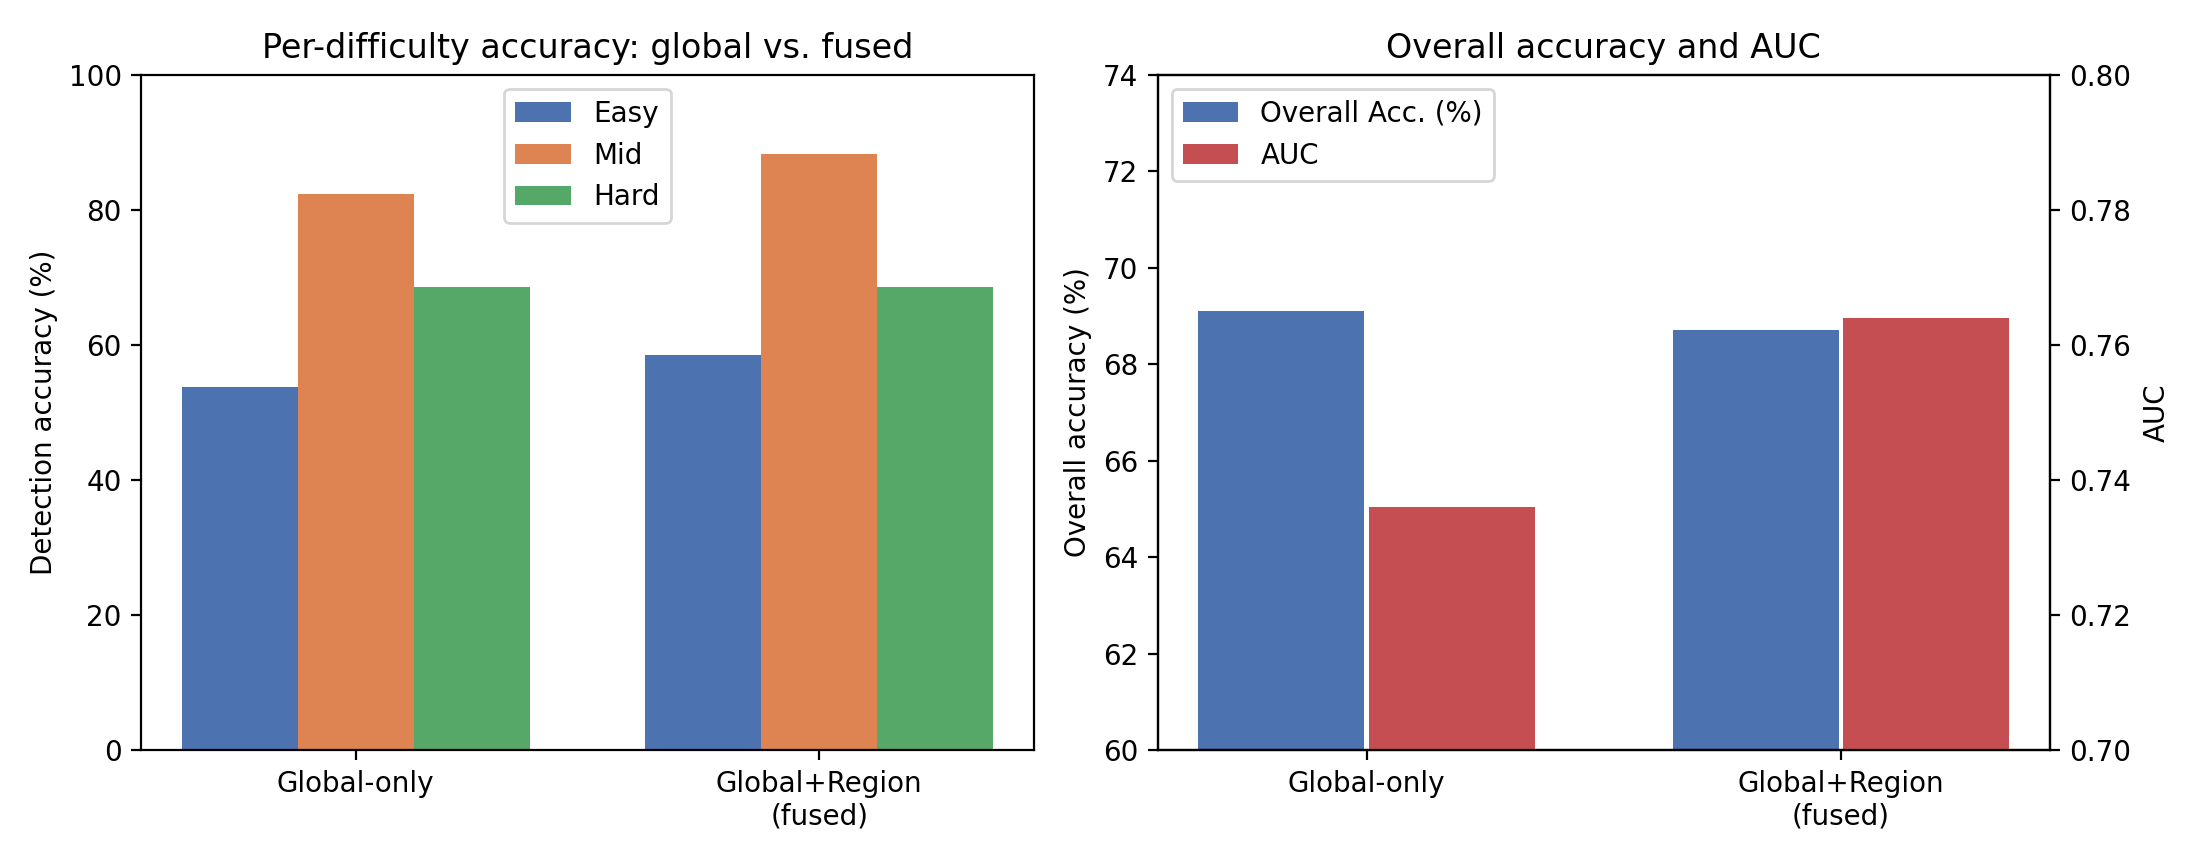
\includegraphics[width=0.95\textwidth]{figures/region_fusion.png}
\caption{Per-difficulty accuracy (left) and overall accuracy/AUC (right) for the global-only vs.\ landmark-based global-plus-region fusion variants.}
\label{fig:regionfusion}
\end{figure}

\subsection{Why the Earlier (Haar-Cascade) Attempt Failed}

This corrected result clarifies why an earlier version of this experiment, using Haar-cascade detection plus fixed anthropometric proportions for region localization, found no improvement. Haar-cascade eye detection is reasonably reliable, but the anthropometric-proportion approach used to place the nose and mouth boxes is a coarse approximation that does not adapt to individual face geometry; for a subtle, spatially confined splice, a loosely or inconsistently cropped ``local'' patch can miss the manipulated region entirely, which effectively degrades the region-local features back into a noisy version of the global signal. Replacing this with MediaPipe FaceMesh's per-landmark localization removes that source of noise and lets the region-local descriptors do what they were designed to do. This is a useful methodological lesson on its own: a negative result for a feature-fusion hypothesis can, in fact, be a positive result for a feature-localization-quality hypothesis, and the two should not be conflated without re-testing at higher localization precision before concluding that a fusion idea simply does not work.

% ============================================================
\section{Cross-Dataset Generalization}
\label{sec:crossdataset}

All results up to this point come from a single source dataset. This section reports the completed test of whether a classifier trained on this corpus's expert-Photoshop-splice attacks generalizes to a mechanistically different, independently sourced presentation-attack corpus.

\subsection{Method}

The classical SVM-RBF pipeline, trained and selected exactly as in Section~5 on the Real-and-Fake-Face-Detection training split, was evaluated --- with no further fitting or adaptation --- against the NUAA Photograph Imposter Database~\cite{tan2010}, a print-attack PAD corpus independent of, and never seen during, training. NUAA's train and test splits were combined into a single held-out target set of 12,611 images (5,105 real, 7,506 print-attack spoof). OULU-NPU, CASIA-FASD, Replay-Attack, and SiW were not used because they require per-user data-use agreements with the releasing institutions that could not be completed in this project's timeframe; NUAA has no such requirement. Evaluation uses the field-standard ISO/IEC 30107-3 metric set (Equation~3) in addition to accuracy and AUC.

\subsection{Results}

\begin{table}[htbp]
\centering
\caption{Cross-dataset generalization: classical SVM-RBF trained on Real-and-Fake-Face-Detection (splice attacks), evaluated zero-shot against NUAA (print attacks).}
\label{tab:crossdataset}
\begin{tabular}{lr}
\toprule
Metric & Value \\
\midrule
Target set size & 12,611 images (5,105 real / 7,506 fake) \\
Accuracy & 40.5\% \\
AUC & 0.507 \\
APCER (attacks misclassified as real) & 99.8\% \\
BPCER (bona fide misclassified as fake) & 0.2\% \\
ACER & 50.0\% \\
\bottomrule
\end{tabular}
\end{table}

\begin{figure}[htbp]
\centering
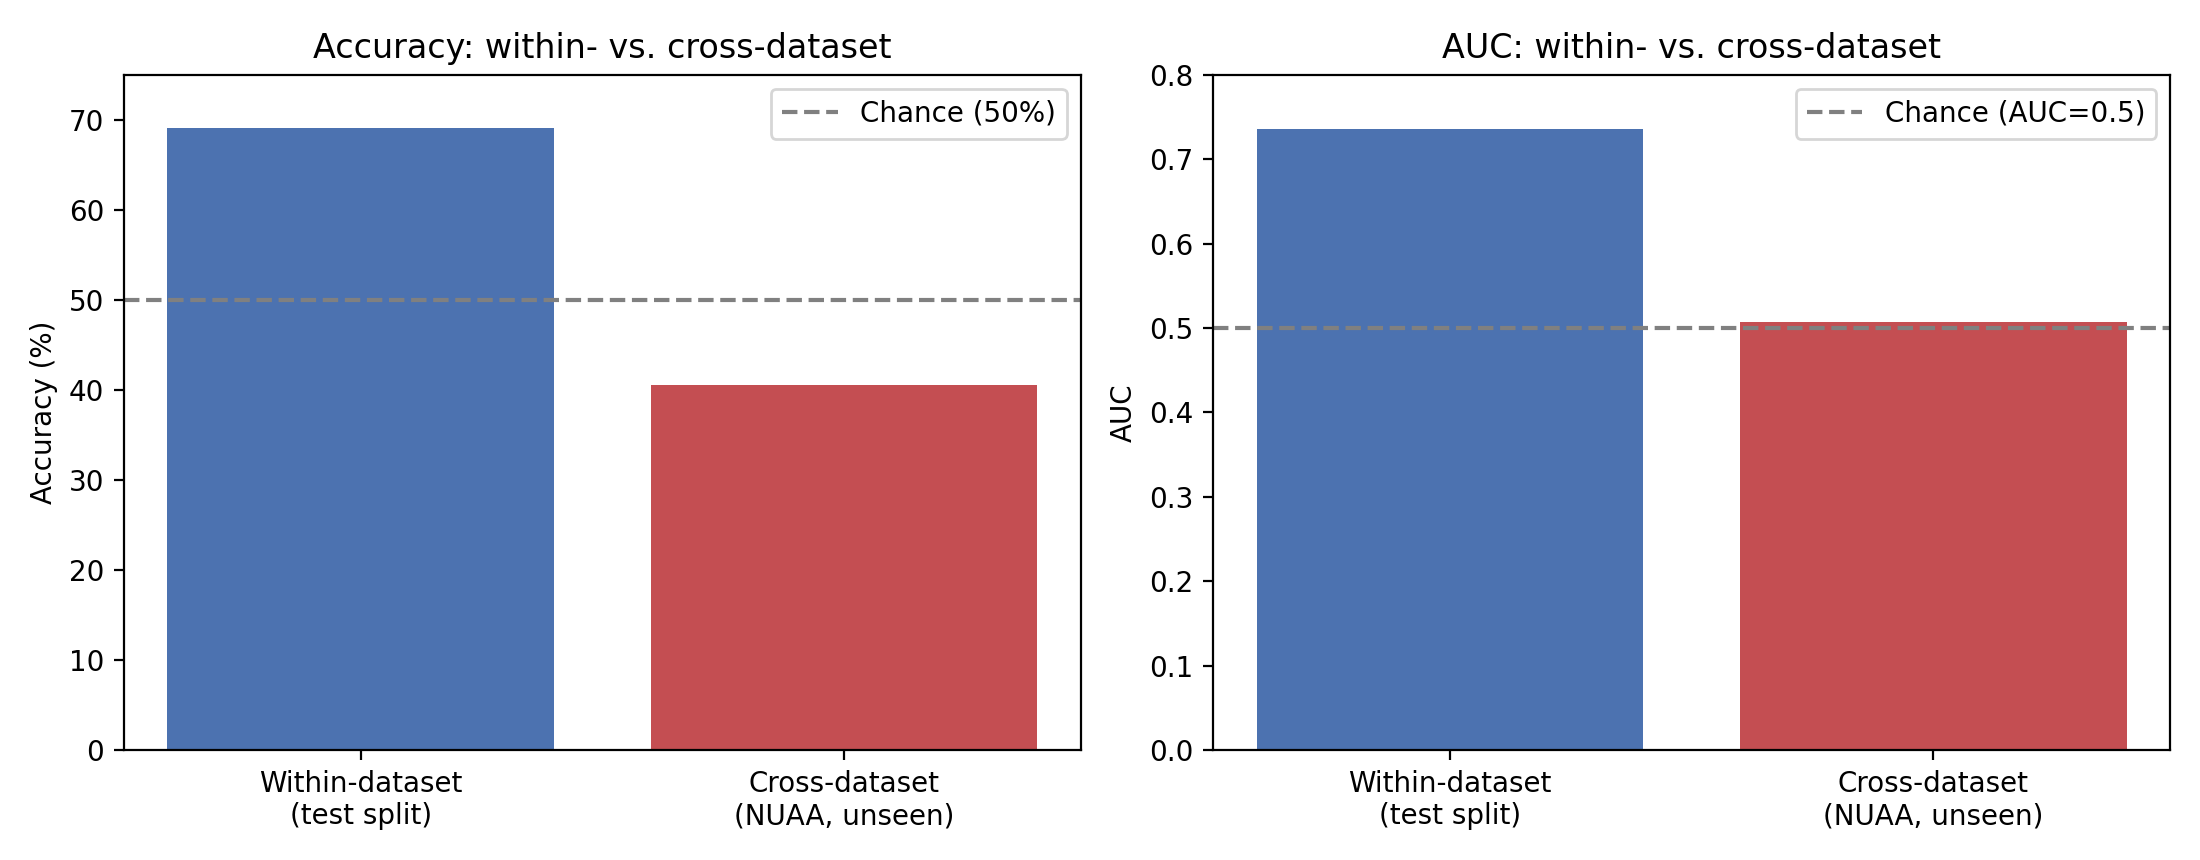
\includegraphics[width=0.95\textwidth]{figures/cross_dataset.png}
\caption{Accuracy and AUC: within-dataset held-out test split vs.\ cross-dataset evaluation against NUAA. The dashed line marks chance-level performance.}
\label{fig:crossdataset}
\end{figure}

The result is unambiguous: 40.5\% accuracy, 0.507 AUC, ACER 50.0\% --- statistically indistinguishable from chance. An APCER of 99.8\% means the model almost never flags a NUAA print-attack image as fake, while a BPCER of 0.2\% means it almost always correctly passes real images; put differently, the model has effectively collapsed to a near-constant ``predict real'' classifier once faced with attack-type distribution shift, rather than genuinely discriminating attack from bona fide in the new domain.

\subsection{Interpretation}

This is exactly what the mechanistic account developed in Section~8 predicts. The classifier's discriminative signal is dominated (92.3\% Gini importance) by HOG features tuned to detect splice-boundary edge discontinuities, a local, high-frequency gradient artifact specific to expert photo compositing. NUAA's spoof images are printed photographs recaptured by a camera, whose defining artifacts are print texture, moir\'e patterning, and color-reproduction shift under recapture --- a global, low-to-mid-frequency color and texture signal, not a localized edge discontinuity. A classifier that learned to detect one artifact type has no mechanistic reason to detect the other, and the near-chance result confirms this directly rather than leaving it as a plausible-sounding hypothesis.

This closes what was previously the central open question in this line of work: does a model trained on one presentation-attack distribution transfer to another? For this pipeline, trained on this dataset, the answer is no. No generalization claim beyond the Real-and-Fake-Face-Detection corpus's specific splice-attack distribution should be drawn from the 69.1\% within-dataset headline number in Section~7; the model's demonstrated applicability is specific to splice/composite-style presentation attacks, not to presentation attacks in general. This is also a useful negative result for the field: it is direct, measured evidence, not an assumption, that print/replay-oriented classical descriptors (LBP, color statistics) and splice-oriented descriptors (HOG, for this dataset) are not interchangeable. That reinforces the motivation in~\cite{boulkenafet2015,boulkenafet2016} for attack-type-aware feature design, but from the opposite direction: a detector over-specialized on one attack type's artifacts should be expected to fail outright, not merely underperform, on another.

% ============================================================
\section{Ethical Considerations}

\subsection{Demographic Fairness}

Liu et al.~\cite{liu2021} document a demographic-fairness gap in PAD generalization across ethnicity, and this paper's dataset does not include demographic labels that would let us run a subgroup-level error analysis. A PAD system with an aggregate false-accept rate of 32.5\% (Section~7) could in principle have that error concentrated disproportionately in specific demographic subgroups without that being visible in any aggregate metric reported here. Any deployment decision informed by this paper's results should not assume uniform error rates across demographic groups without a dedicated fairness evaluation.

\subsection{Consent, Provenance, and Licensing}

The dataset used here is CIPLAB/Yonsei University's publicly available Real and Fake Face Detection corpus, licensed CC-BY-NC-SA-4.0, which requires attribution to the creators, restricts use to non-commercial purposes, and requires any redistributed derivative of the dataset itself to carry the same license. Because the ``fake'' class is composed of expert Photoshop composites splicing regions from different real individuals' photographs, users of this dataset should also consider whether the original data-collection and compositing process obtained appropriate consent for the specific derivative uses --- including PAD research --- to which the resulting images are subsequently put.

\subsection{Dual-Use Considerations}

PAD research is inherently dual-use: detection techniques could, in principle, inform an adversary's efforts to build spoofs specifically engineered to evade a known detector. This paper reports only detection-side results and offers no attack-optimization guidance; the cross-dataset negative result of Section~12, for instance, is reported because it is scientifically informative about detector limitations and the risk of over-generalizing a single-dataset accuracy figure, not as guidance for attack construction.

\subsection{Deployment Responsibility}

Given the modest within-dataset accuracy ceiling (a raw error rate of 31\% for the best classical model) and the demonstrated chance-level cross-dataset generalization (Section~12), any real-world deployment built on this exact pipeline should treat its decision as one signal among several --- combined with a second biometric factor or a human-reviewed fallback --- rather than as a sole, automated access-control gate, and it should not be deployed against attack types (printed-photo or video replay, for instance) outside the splice/composite distribution it was trained and validated on.

% ============================================================
\section{Discussion and Limitations}

\subsection{Cross-Dataset Generalization: Now Measured, Not Assumed}

An earlier draft of this study flagged cross-dataset generalization as the single largest open question and left it as future work. This revision closes that gap directly (Section~12): the model does not generalize to a mechanistically different attack type, and that is now a measured finding rather than a caveat.

\subsection{Single-Attack-Type Training Data}

The Real-and-Fake-Face-Detection corpus contains only expert-composited splice attacks. That is the direct cause of the cross-dataset failure in Section~12: a model can only learn to detect the artifact types present in its training distribution. A materially larger and/or multi-source, multi-attack-type training corpus (splice, print, replay, and 3D mask) would be needed before a broader generalization claim could be supported.

\subsection{Small, Single-Source Dataset}

At 2,041 images, this corpus is two to three orders of magnitude smaller than standard deep-PAD training sets (Section~4), which limits what any model, classical or deep, can realistically learn here.

\subsection{Static Images Only}

No temporal or depth information is used, so this pipeline cannot exploit motion or liveness cues such as blinking, micro-motion, or pulse signals extracted via rPPG, which dominate modern state-of-the-art PAD systems~\cite{liu2018}.

\subsection{Region Localization Quality Matters}

Section~11 showed that the region-local fusion hypothesis's apparent failure in an earlier attempt was a localization-quality artifact, not evidence against the hypothesis itself. This is a general caution for any patch-based or region-local PAD method: a negative fusion result should not be trusted until region localization has been validated at adequate precision.

\subsection{The ``Fake'' Class Is a Third Category}

Per Tolosana et al.~\cite{tolosana2020}, the PAD literature usually distinguishes physical presentation attacks from digital GAN-based deepfakes. This dataset's ``fake'' class is neither: it is not a photograph of a physical presentation medium, nor a GAN-synthesized image, but a manually composited splice of real photographic regions. Results here should be read as evidence about detecting expert-composited digital face manipulation using color-texture descriptors, and the cross-dataset result in Section~12 should be read as evidence that this is a distinct detection problem from print/replay PAD, not a subset or superset of it.

\subsection{Summary of Limitations}

\begin{table}[htbp]
\centering
\caption{Summary of limitations and mitigations.}
\label{tab:limitations}
\small
\begin{tabular}{p{3.6cm}p{4.2cm}p{5.0cm}}
\toprule
Limitation & Potential impact & Mitigation \\
\midrule
Single-attack-type training data & Does not generalize to print/replay/mask attacks & Measured directly (Section~12); flagged as precondition for broader deployment \\
Small, single-source data & Limits both classical and deep model ceiling & Explicit scale comparison (Section~4) \\
Static images only & Misses motion/rPPG liveness cues & Flagged as future extension \\
No demographic fairness data & Unknown subgroup error rates & Flagged as deployment precondition \\
``Fake'' class terminology & Conflates PAD and deepfake/splice detection & Corrected provenance and explicit scoping caveat (this section) \\
\bottomrule
\end{tabular}
\end{table}

Taken together, this project is a statistically validated re-evaluation of a classical color-texture PAD pipeline on one modest, single-attack-type dataset, with a controlled ablation identifying which feature family carries the signal, a directly executed deep-learning comparison, a corrected and re-executed region-local fusion experiment with a genuine positive result, and a directly executed cross-dataset generalization test with a genuine, cautionary negative result. Recent classical-descriptor PAD papers~\cite{gunay2023,chang2022} show this remains a publishable genre in student-track and workshop venues when framed this way. This project is not a claim of state-of-the-art or competitive performance against modern deep PAD systems, and it is not a generalization claim beyond the specific attack type it was trained and tested on --- a boundary this revision now demonstrates empirically rather than merely acknowledges. As scoped, it is not ready for a mainstream computer-vision or biometrics venue such as CVPR, ICCV, IJCB, or BTAS; that would require a materially larger, multi-source, multi-attack-type training corpus.

% ============================================================
\section{Conclusion and Future Work}

This paper presented a classical color-texture face anti-spoofing pipeline evaluated with a level of rigor --- controlled ablation, bootstrap and repeated-split significance testing, a data-budget-matched deep-learning comparison, a corrected and re-executed region-local fusion experiment, and a completed cross-dataset generalization test --- that is uncommon in student and portfolio-level PAD projects. The best classical model, SVM-RBF, reaches 69.1\% accuracy and 0.736 AUC on held-out data from its training distribution, and it outperforms a fine-tuned MobileNetV2 baseline on the identical split by a substantial margin, showing that at a roughly 1,400-image training budget, hand-crafted color-texture features remain a legitimate, and here a stronger, choice than a lightly fine-tuned CNN. A controlled ablation shows that HOG alone accounts for nearly all of the fused pipeline's discriminative power on this dataset, now correctly attributed to splice-boundary edge detection rather than a generic ``GAN artifact.'' A re-executed, landmark-based region-local feature-fusion experiment shows that the model's easy-attack blind spot can be partly closed by adding local eye, nose, and mouth descriptors, provided region localization is precise enough --- correcting an earlier negative finding that was actually a localization-quality artifact. Finally, a completed cross-dataset test against an independent print-attack corpus (NUAA) shows the model performing at chance outside the splice-attack distribution it was trained on, closing the central open question of this line of work with a genuine, informative negative result rather than leaving it as unexecuted future work.

\subsection{Priority-Ordered Future Work}

\begin{enumerate}
\item \textbf{Multi-attack-type training data.} Given Section~12's finding that a splice-trained classifier fails on print attacks, the most valuable next step is training on a combined, multi-attack-type corpus (splice + print + replay, subject to data-use agreements for OULU-NPU, CASIA-FASD, Replay-Attack, or SiW) to test whether a fused classifier can learn attack-type-invariant liveness cues rather than artifact-specific ones.
\item \textbf{Attack-type-aware or ensemble detection.} Given that HOG (splice-tuned) and LBP/color (print/replay-tuned, per the original Boulkenafet et al.\ motivation) appear to specialize in mutually exclusive artifact types, an ensemble or attack-type classifier stage that routes to a specialized detector may outperform a single fused model trained across attack types.
\item \textbf{Demographic fairness evaluation.} Where a dataset with demographic annotations can be obtained under appropriate data-use terms, extend the per-difficulty error analysis to per-subgroup error rates.
\item \textbf{Video-based extension.} Incorporate a video-replay attack subtype and temporal descriptors (frame-difference texture, or a lightweight rPPG estimator) to test whether this pipeline's static-image blind spot to replay attacks is real, and whether it compounds with the attack-type generalization gap measured here.
\item \textbf{Isolate the classical-vs-deep gap's root cause.} A controlled study varying pretraining source, backbone capacity, and fine-tuning depth independently would isolate which factor dominates MobileNetV2's underperformance on this data budget.
\end{enumerate}

% ============================================================
\appendix
\section{Hyperparameter Grids and Best Configurations}

\begin{table}[htbp]
\centering
\caption{Hyperparameter grids and cross-validation-selected best configuration.}
\label{tab:hyperparams}
\begin{tabular}{lll}
\toprule
Model & Grid searched & Best configuration (5-fold CV, F1) \\
\midrule
Logistic Regression & $C\in\{0.1,1,10\}$ & $C=1$ \\
SVM (RBF) & $C\in\{1,10,50\}$, $\gamma\in\{\text{scale},0.01\}$ & $C=1$, $\gamma=\text{scale}$ \\
Random Forest & $n_{\text{est}}\in\{200,400\}$, depth$\in\{\text{None},20\}$ & $n_{\text{est}}=200$, depth=None \\
\bottomrule
\end{tabular}
\end{table}

\section{Reproducibility Checklist}

\textbf{Code availability.} All scripts referenced in this paper (\texttt{build\_dataset.py}, \texttt{build\_dataset\_region.py}, \texttt{train\_evaluate.py}, \texttt{ablation\_study.py}, \texttt{statistical\_significance.py}, \texttt{deep\_baseline\_mobilenetv2.py}, \texttt{region\_features.py}, \texttt{train\_hybrid\_fusion.py}, \texttt{train\_score\_fusion.py}, \texttt{cross\_dataset\_eval.py}) are available at \url{https://github.com/Sandilya-17/Face-antispoofing.git}.

\textbf{Random seeds.} The main pipeline uses a fixed seed (\texttt{random\_state=42}) for the train/validation/test split and all classifier initialization. The repeated-split experiment (Section~9) explicitly varies this seed across $i=1,\ldots,30$.

\textbf{Data splits.} Fixed 70/15/15 stratified split by class label, sizes given in Table~\ref{tab:splits}.

\textbf{Search protocol.} 5-fold stratified cross-validation on the training split only, grid search optimizing F1; full grids in Table~\ref{tab:hyperparams}.

\textbf{Evaluation protocol.} Each model's cross-validation-selected configuration is refit once on the full training split and evaluated exactly once on the held-out test split; no test-set information is used during model selection.

\textbf{Software versions.} Python 3.10, scikit-learn, scikit-image, OpenCV, MediaPipe, TensorFlow/Keras (with \texttt{tensorflow-metal} for GPU acceleration), SciPy.

\textbf{Status of all experiments in this revision.} Main classical pipeline: executed. Ablation: executed. Statistical significance: executed. Deep-learning baseline: executed (GPU). Region-local fusion: executed with landmark-based localization (positive result); an earlier Haar-cascade-based attempt is documented as superseded. Cross-dataset evaluation: executed against NUAA (negative/chance-level result). No claim in this paper depends on an unexecuted experiment.

% ============================================================
\begin{thebibliography}{99}

\bibitem{ojala2002} T. Ojala, M. Pietik\"ainen, and T. M\"aenp\"a\"a, ``Multiresolution gray-scale and rotation invariant texture classification with local binary patterns,'' \emph{IEEE Trans. Pattern Anal. Mach. Intell.}, vol.\ 24, no.\ 7, pp.\ 971--987, 2002.

\bibitem{dalal2005} N. Dalal and B. Triggs, ``Histograms of oriented gradients for human detection,'' in \emph{Proc. IEEE Conf. Computer Vision and Pattern Recognition (CVPR)}, 2005, pp.\ 886--893.

\bibitem{boulkenafet2015} Z. Boulkenafet, J. Komulainen, and A. Hadid, ``Face anti-spoofing based on color texture analysis,'' in \emph{Proc. IEEE Int. Conf. Image Processing (ICIP)}, 2015, pp.\ 2636--2640.

\bibitem{boulkenafet2016} Z. Boulkenafet, J. Komulainen, and A. Hadid, ``Face spoofing detection using colour texture analysis,'' \emph{IEEE Trans. Inf. Forensics Security}, vol.\ 11, no.\ 8, pp.\ 1818--1830, 2016.

\bibitem{chingovska2012} I. Chingovska, A. Anjos, and S. Marcel, ``On the effectiveness of local binary patterns in face anti-spoofing,'' in \emph{Proc. Int. Conf. Biometrics Special Interest Group (BIOSIG)}, 2012, pp.\ 1--7.

\bibitem{zhang2012} Z. Zhang, J. Yan, S. Liu, Z. Lei, D. Yi, and S. Z. Li, ``A face antispoofing database with diverse attacks,'' in \emph{Proc. IAPR Int. Conf. Biometrics (ICB)}, 2012, pp.\ 26--31.

\bibitem{boulkenafet2017} Z. Boulkenafet et al., ``OULU-NPU: A mobile face presentation attack database with real-world variations,'' in \emph{Proc. IEEE Int. Conf. Automatic Face \& Gesture Recognition (FG)}, 2017, pp.\ 612--618.

\bibitem{liu2018} Y. Liu, A. Jourabloo, and X. Liu, ``Learning deep models for face anti-spoofing: Binary or auxiliary supervision,'' in \emph{Proc. IEEE Conf. Computer Vision and Pattern Recognition (CVPR)}, 2018, pp.\ 389--398.

\bibitem{jourabloo2018} A. Jourabloo, Y. Liu, and X. Liu, ``Face de-spoofing: Anti-spoofing via noise modeling,'' in \emph{Proc. European Conf. Computer Vision (ECCV)}, 2018, pp.\ 290--306.

\bibitem{atoum2017} Y. Atoum, Y. Liu, A. Jourabloo, and X. Liu, ``Face anti-spoofing using patch and depth-based CNNs,'' in \emph{Proc. IEEE Int. Joint Conf. Biometrics (IJCB)}, 2017, pp.\ 319--328.

\bibitem{george2019} A. George and S. Marcel, ``Deep pixel-wise binary supervision for face presentation attack detection,'' in \emph{Proc. IAPR Int. Conf. Biometrics (ICB)}, 2019, pp.\ 1--8.

\bibitem{yu2020} Z. Yu et al., ``Searching central difference convolutional networks for face anti-spoofing,'' in \emph{Proc. IEEE Conf. Computer Vision and Pattern Recognition (CVPR)}, 2020, pp.\ 5295--5305.

\bibitem{qin2020} Y. Qin et al., ``Learning meta model for zero- and few-shot face anti-spoofing,'' in \emph{Proc. AAAI Conf. Artificial Intelligence}, 2020, pp.\ 11916--11923.

\bibitem{wang2020} Y. Wang et al., ``CelebA-Spoof: Large-scale face anti-spoofing dataset with rich annotations,'' in \emph{Proc. European Conf. Computer Vision (ECCV)}, 2020, pp.\ 70--85.

\bibitem{jia2020} S. Jia, G. Guo, and Z. Xu, ``A survey on 3D mask presentation attack detection and countermeasures,'' \emph{Pattern Recognit.}, vol.\ 98, p.\ 107032, 2020.

\bibitem{tolosana2020} R. Tolosana, R. Vera-Rodriguez, J. Fierrez, A. Morales, and J. Ortega-Garcia, ``Deepfakes and beyond: A survey of face manipulation and fake detection,'' \emph{Inf. Fusion}, vol.\ 64, pp.\ 131--148, 2020.

\bibitem{liu2021} A. Liu et al., ``Cross-ethnicity face anti-spoofing recognition challenge: A review,'' \emph{IET Biometrics}, vol.\ 10, no.\ 1, pp.\ 24--43, 2021.

\bibitem{heusch2020} G. Heusch, A. George, D. Geissb\"uhler, Z. Mostaani, and S. Marcel, ``Deep models and shortwave infrared information to detect face presentation attacks,'' \emph{IEEE Trans. Biometrics, Behavior, and Identity Science}, vol.\ 2, no.\ 4, pp.\ 399--409, 2020.

\bibitem{yu2023} Z. Yu, Y. Qin, X. Li, C. Zhao, Z. Lei, and G. Zhao, ``Deep learning for face anti-spoofing: A survey,'' \emph{IEEE Trans. Pattern Anal. Mach. Intell.}, vol.\ 45, no.\ 5, pp.\ 5609--5631, 2023.

\bibitem{gunay2023} A. G\"unay Y\i lmaz, U. Turhal, and V. Nabiyev, ``Face presentation attack detection performances of facial regions with multi-block LBP features,'' \emph{Multimedia Tools Appl.}, vol.\ 82, pp.\ 30587--30606, 2023.

\bibitem{chang2022} H.-H. Chang and C.-H. Yeh, ``Face anti-spoofing detection based on multiscale image quality assessment,'' \emph{Image Vis. Comput.}, vol.\ 121, p.\ 104428, 2022.

\bibitem{biswas2025} A. S. Biswas, S. Dey, S. Verma, and K. Verma, ``DeepGuard: An enhanced hybrid ensemble classifier for face presentation attack detection integrating Gabor and binarized statistical image features descriptors with deep learning,'' \emph{Comput. Electr. Eng.}, vol.\ 127, p.\ 110560, 2025.

\bibitem{pinto2020} A. Pinto, S. Goldenstein, A. Ferreira, T. Carvalho, H. Pedrini, and A. Rocha, ``Leveraging shape, reflectance and albedo from shading for face presentation attack detection,'' \emph{IEEE Trans. Inf. Forensics Security}, vol.\ 15, pp.\ 3347--3358, 2020.

\bibitem{hernandez2019} J. Hernandez-Ortega, J. Fierrez, A. Morales, and J. Galbally, ``Introduction to face presentation attack detection,'' in \emph{Handbook of Biometric Anti-Spoofing}, Springer, 2019, pp.\ 187--206.

\bibitem{tan2010} X. Tan, Y. Li, J. Liu, and L. Jiang, ``Face liveness detection from a single image with sparse low rank bilinear discriminative model,'' in \emph{Proc. European Conf. Computer Vision (ECCV)}, 2010, pp.\ 504--517. (NUAA Photograph Imposter Database.)

\end{thebibliography}

\end{document}
